\documentclass[a4paper, twoside]{article}

\usepackage{lipsum} % genera testo fittizio
\usepackage{amsmath} % visualizzazione matrici
\usepackage{pdfpages}

% FONT %
\usepackage[T1]{fontenc}
\usepackage[utf8]{inputenc}
\usepackage{tgschola}
\usepackage[fontsize=12pt]{scrextend}
\linespread{1.25}

% IMPAGINAZIONE %
\usepackage[english,italian]{babel}
\usepackage[a4paper,top=3cm,bottom=3cm,left=3cm,right=3cm]{geometry}
\raggedbottom % lascia spazio alla fine delle pagine

% HEADER & FOOTER %
\usepackage{fancyhdr}
\usepackage[bottom]{footmisc}
\setlength{\headheight}{14.5pt}
\pagestyle{fancy}
\fancypagestyle{plain}{\renewcommand{\headrulewidth}{0pt}\fancyhf{}}

% IMMAGINI %
\usepackage{graphicx}
\usepackage{caption}
\usepackage{subcaption}
\usepackage{float}
\usepackage{amsmath}
\graphicspath{{./images/}}

% BLOCCHI DI CODICE %
\usepackage{xcolor}
\definecolor{bgTitleCode}{RGB}{12,44,64}
\usepackage[ttdefault=true]{AnonymousPro}
\usepackage{listings}
\usepackage{minted}
\usepackage{tcolorbox}
\tcbuselibrary{listings, breakable, minted, skins}
\tcbset{listing engine=minted}

\newtcblisting{tsxCode}[2][]{
    breakable,
    listing only, #1 ,title=#2,
    minted language=html,
    minted style=vs,
    coltitle=white,
    colbacktitle=bgTitleCode,
    toptitle=3mm, bottomtitle=2.5mm,
    top=2mm, bottom=3mm,
    fonttitle=\ttfamily,
    enhanced, frame hidden, 
    minted options={fontfamily=AnonymousPro,
    fontsize=\footnotesize, tabsize=2,
    breaklines, breaksymbolleft=\hspace{1em}
    ,autogobble, linenos=false}}

\newtcblisting{tsCode}[2][]{
    breakable,
    listing only, #1 ,title=#2,
    minted language=ts,
    minted style=vs,
    coltitle=white,
    colbacktitle=bgTitleCode,
    toptitle=3mm, bottomtitle=2.5mm,
    top=2mm, bottom=3mm,
    fonttitle=\ttfamily,
    enhanced, frame hidden, 
    minted options={fontfamily=AnonymousPro,
    fontsize=\scriptsize, tabsize=2,
    breaklines, breaksymbolleft=\hspace{1em}
    ,autogobble, linenos=false}}

\newtcblisting{pyCode}[2][]{
    breakable,
    listing only, #1 ,title=#2,
    minted language=python,
    minted style=vs,
    coltitle=white,
    colbacktitle=bgTitleCode,
    toptitle=3mm, bottomtitle=2.5mm,
    top=2mm, bottom=3mm,
    fonttitle=\ttfamily,
    enhanced, frame hidden, 
    minted options={fontfamily=AnonymousPro,
    fontsize=\scriptsize, tabsize=2,
    breaklines, breaksymbolleft=\hspace{1em}
    ,autogobble, linenos=false}}

% BIBLIOGRAFIA %
\usepackage{csquotes}
\usepackage[style=alphabetic, sorting=ynt]{biblatex}
\DeclareUnicodeCharacter{0394}{$\Delta$}
\addbibresource{tex/bibliography.bib}

% LINK ESTERNI %
\newcommand\anchor[2]{\href{#2}{#1}\footnote{\hspace{.2em}\url{#2}}}

\definecolor{linkColor}{RGB}{2,11,120}
\definecolor{printLinkColor}{RGB}{0,0,0}
\usepackage[colorlinks=true, allcolors=printLinkColor]{hyperref}


% INIZIO DOCUMENTO %

\begin{document}

% TITOLO %
\fancyhf{} % reset header & footer
\begin{titlepage}
\begin{figure}[H]
    \centering
    
\includegraphics[width=7cm]{images/unifi.png}
\end{figure}

\begin{center}
    \LARGE{UNIVERSITÀ DI FIRENZE}
    \vspace{1mm}
    \\ \large{DIPARTIMENTO DI INFORMATICA }
    \vspace{5mm}
    \\ \LARGE{Corso di Laurea Triennale in \\[-1mm] Ingegneria Informatica}
\end{center}

\vspace{15mm}
\begin{center}\LARGE\textbf{Frontend per la simulazione \\[-0.1em] di platooning di veicoli}
\end{center}
\vspace{30mm}

\begin{minipage}[t]{0.47\textwidth}
	{\large{Relatore}{\normalsize\vspace{3mm}
	\bf\\ \large{Giorgio Battistelli}}}
\end{minipage}
\hfill
\begin{minipage}[t]{0.47\textwidth}\raggedleft
	{\large{Candidati}{\normalsize\vspace{3mm}
	\bf\\ \large{Federico Marra \vspace{2mm}\\Alberto Del Buono Paolini}}}
\end{minipage}

\end{titlepage}

% INDICE %
\newpage
\fancyhead[RO,LE]{Indice}
\tableofcontents

% FOOTER CON NUMERO %
\newpage
\fancyfoot[RO,LE]{\thepage}
\setcounter{page}{1}

% CAPITOLI %
\section{Introduzione}
\fancyhead[RO,LE]{Introduzione}

La crescita del traffico stradale e la capacità limitata delle infrastrutture autostradali rappresentano sfide sempre più pressanti per le società moderne. L'incremento costante del numero di veicoli in circolazione ha portato a una saturazione sempre maggiore delle strade, ma anche a un aumento della durata degli spostamenti, con conseguenti ritardi, stress per gli automobilisti e impatti negativi sull'ambiente dovuti alle emissioni generate dal traffico fermo. In questo contesto, la ricerca di soluzioni innovative e efficienti per migliorare la gestione del traffico stradale è diventata sempre più importante.
\newline
Tra le molteplici strategie proposte per affrontare questo problema, una delle più promettenti è il concetto di platooning di veicoli. Detto anche convogliamento, consiste nell'allineamento e nella gestione coordinata di più veicoli in movimento lungo una strada. Questa formazione di veicoli segue un veicolo guida, cercando di mantenere una distanza costante prestabilita e ridotta tra di loro e minore in confronto alla distanza di si, e risponde in modo coordinato alle variazioni di velocità e direzione del veicolo di testa. Questo approccio offre numerosi vantaggi, tra cui una maggiore efficienza nel flusso del traffico, una riduzione della distanza tra i veicoli stessi e un miglioramento della sicurezza stradale.
\newline
Tuttavia, la piena realizzazione del potenziale del platooning richiede l'adozione di sistemi avanzati di controllo e automazione dei veicoli. In particolare, è fondamentale sviluppare algoritmi e tecnologie in grado di coordinare in modo efficace e sicuro il movimento dei veicoli all'interno del convoglio, garantendo contemporaneamente il rispetto delle normative stradali e la massima sicurezza per i conducenti e gli altri utenti della strada.
\newline
A questo scopo, il controllo di crociera adattivo e cooperativo (CACC) si presenta come una soluzione promettente. Questo sistema utilizza dati provenienti dai veicoli stessi, oltre a informazioni ottenute da sensori come telecamere, radar e lidar (scanner laser), per regolare automaticamente la velocità e la distanza tra i veicoli all'interno del convoglio. Grazie alla sua capacità di scambio di dati wireless tra veicoli, il CACC consente di mantenere intervalli di tempo significativamente inferiori rispetto ai sistemi di controllo di crociera adattivi tradizionali, contribuendo così a aumentare la capacità delle strade e a ridurre il consumo di carburante.
\newline
Da annoverare fra i vantaggi bisogna vagliare il caso in cui ci sia bisogno di frenare bruscamente, se c'è una persona alla guida c'è da tenere conto del tempo di reazione, calcolato mediamente in un range fra $1s$ e $1.1s$ che corrisponde però a una distanza maggiore proporzionalmente alla velocità a cui si sta viaggiando, come mostrato in figura:
\begin{figure}[H]
    \centering
    \captionsetup{justification=centering, margin=2cm}
    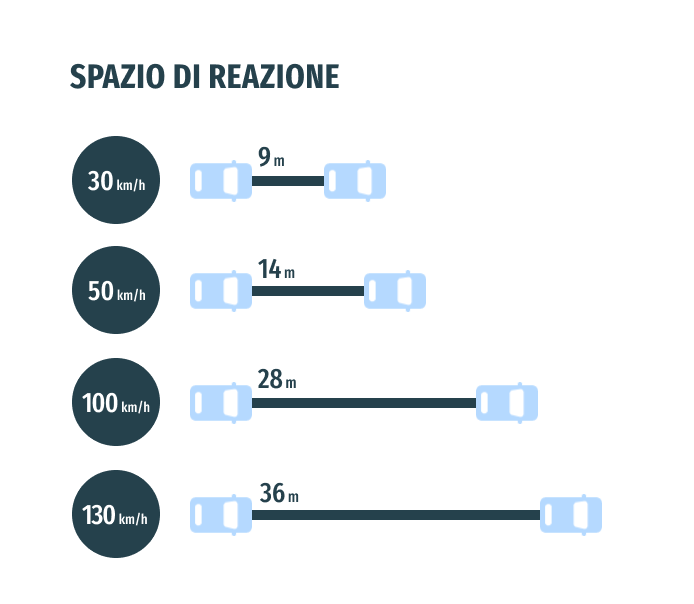
\includegraphics[width=0.75\textwidth]{images/1-introduction/spazio-reazione.png}
    \caption{Spazio di reazione di un veicolo con guidatore umano con tempo di reazione $1s$ \cite{distanza_sicurezza_autoscuola_quattroruote}}
    \label{fig:spazio-reazione}
\end{figure}
\noindent quindi considerando anche lo spazio di frenatura come mostrato in figura

\begin{figure}[H]
    \centering
    \captionsetup{justification=centering, margin=2cm}
    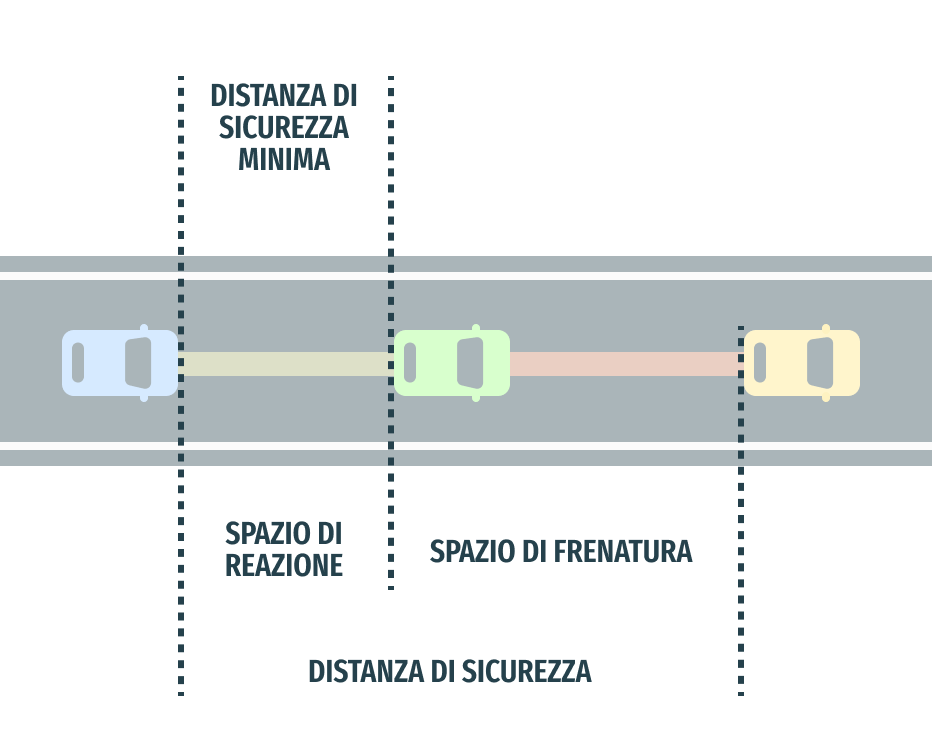
\includegraphics[width=0.8\textwidth]{images/1-introduction/distanze-sicurezza-spazi.png}
    \caption{Componenti distanza di sicurezza \cite{distanza_sicurezza_patentino_online}}
    \label{fig:distanze-sicurezza-spazi}
\end{figure}

\noindent Tuttavia, nonostante i suoi evidenti vantaggi, l'implementazione efficace del CACC e dei sistemi di platooning richiede la progettazione e lo sviluppo di un frontend sofisticato e efficiente per la simulazione e la valutazione delle prestazioni di tali sistemi. È qui che il nostro progetto entra in gioco. Ci proponiamo di sviluppare un frontend innovativo per la simulazione del platooning di veicoli, concentrandoci sull'ottimizzazione del modello fisico e del sistema di controllo, al fine di massimizzare l'efficienza del traffico stradale, garantendo al contempo la massima sicurezza per tutti gli utenti della strada.

\begin{figure}[H]
    \centering
    \captionsetup{justification=centering, margin=2cm}
    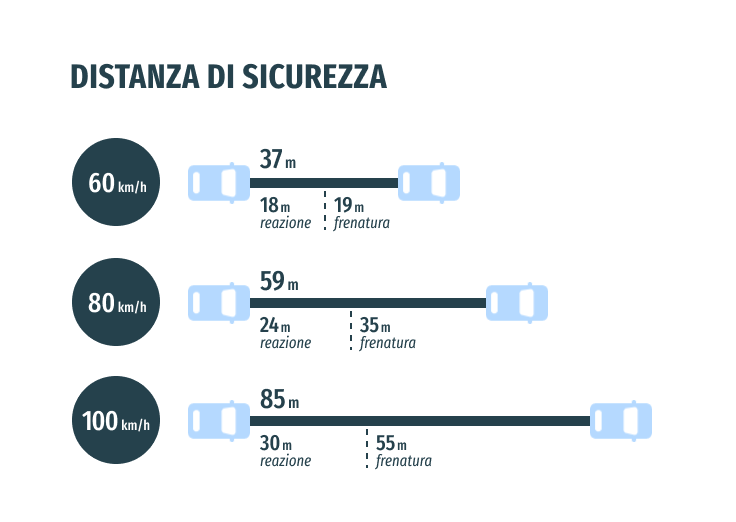
\includegraphics[width=0.8\textwidth]{images/1-introduction/distanza-sicurezza.png}
    \caption{Distanza di sicurezza \cite{distanza_sicurezza_autoscuola_quattroruote}}
    \label{fig:distanza-sicurezza}
\end{figure}

\newpage
\section{Platooning di veicoli}
\fancyhead[RO,LE]{Platooning di veicoli}

Utilizziamo il metodo descritto nell'articolo \cite{ploeg_2014_lp}.


\subsection{Modello matematico del platooning}

\begin{figure}[H]
    \centering
    \captionsetup{justification=centering, margin=2cm}
    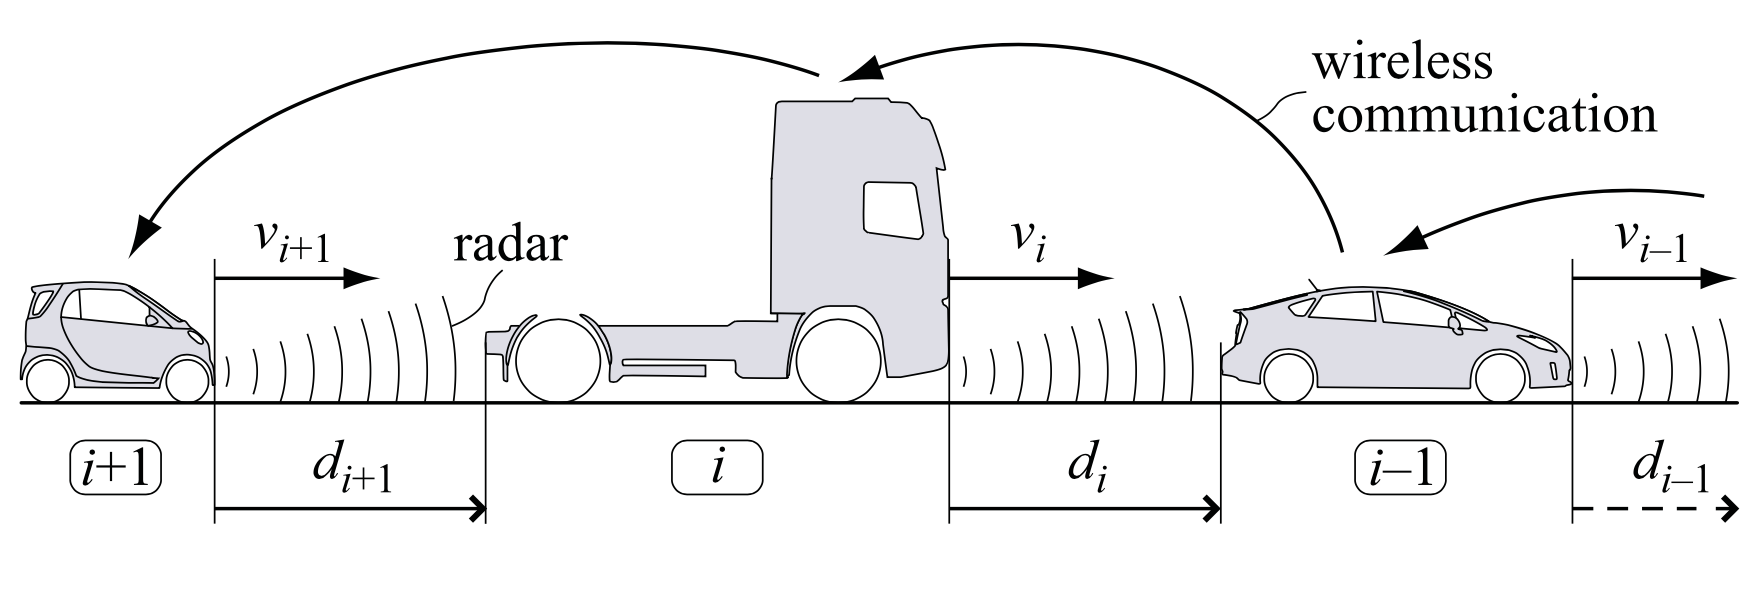
\includegraphics[width=\textwidth]{images/2-theory/PWN-CACC-equipped-vehicle-platoon.png}
    \caption{Platoon di veicoli equipaggiati con CACC}
    \label{fig:cacc-vehicle}
\end{figure}

\newpage
\subsection{Equazioni in forma matriciale}
% Matrici platoon
$\begin{bmatrix}
    \Dot{e}_i \\
    \Dot{v}_i \\
    \Dot{a}_i \\
    \Dot{u}_i
\end{bmatrix}$ = 
$\begin{bmatrix}
    0 & -1 & -h & 0 \\
    0 & 0 & 1 & 0 \\
    0 & 0 & -\frac{1}{\tau} & \frac{1}{\tau} \\
    \frac{k_p}{h} & -\frac{k_d}{h} & -k_d-\frac{k_{dd}(\tau-h)}{h\tau} & -\frac{k_{dd}h+\tau}{h\tau}
\end{bmatrix}$ · 
$\begin{bmatrix}
    e_i \\
    v_i \\
    a_i \\
    u_i
\end{bmatrix}$ +
$\begin{bmatrix}
    0 & 1 & 0 & 0 \\
    0 & 0 & 0 & 0 \\
    0 & 0 & 0 & 0 \\
    0 & \frac{k_d}{h} & \frac{k_{dd}}{h} & \frac{1}{h} \\
\end{bmatrix}$ · 
$\begin{bmatrix}
    e_{i-1} \\
    v_{i-1} \\
    a_{i-1} \\
    u_{i-1}
\end{bmatrix}$
\newline
\newline
Riassunta: $\Dot{x}_i = A_0x_i + A_1x_{i-1}$
con $x_i = (e_i, v_i, a_i, u_i)^t$ che rappresenta il vettore allo stato $i$.

\noindent Svolgiamo il prodotto fra matrici trascurando il fattore $k_{dd}$ che poniamo a $0$ e otteniamo:
\newline

\noindent L'errore: \(\Dot{e}_i = -v_i - ha_i + v_{i-1}\)
\newline

\noindent La velocità: \(\Dot{v}_i = a_i\)
\newline

\noindent L'accelerazione: \(\Dot{a}_i = -\frac{a_i}{\tau} + \frac{u_i}{\tau} = \frac{-a_i+u_i}{\tau}\)
\newline

\noindent Il controllo: \(\Dot{u}_i = \frac{k_p}{h}e_i -\frac{k_d}{h}v_i - k_da_i - \frac{u_i}{h} + \frac{k_d}{h}v_{i-1} + \frac{u_{i-1}}{h} = \frac{k_pe_i - k_dv_i - u_i + k_dv_{i-1} + u_{i-1}}{h} - k_da_i\)

\newpage
\subsection{Campionamento e discretizzazione delle equazioni}

%STAND-ALONE EQUATION EXAMPLE
%\[ x^n + y^n = z^n \]
\newpage
\section{Simulazione del platooning}
\fancyhead[RO,LE]{Simulazione del platooning}

\subsection{Implementazione della simulazione}

\begin{figure}[H]
    \centering
    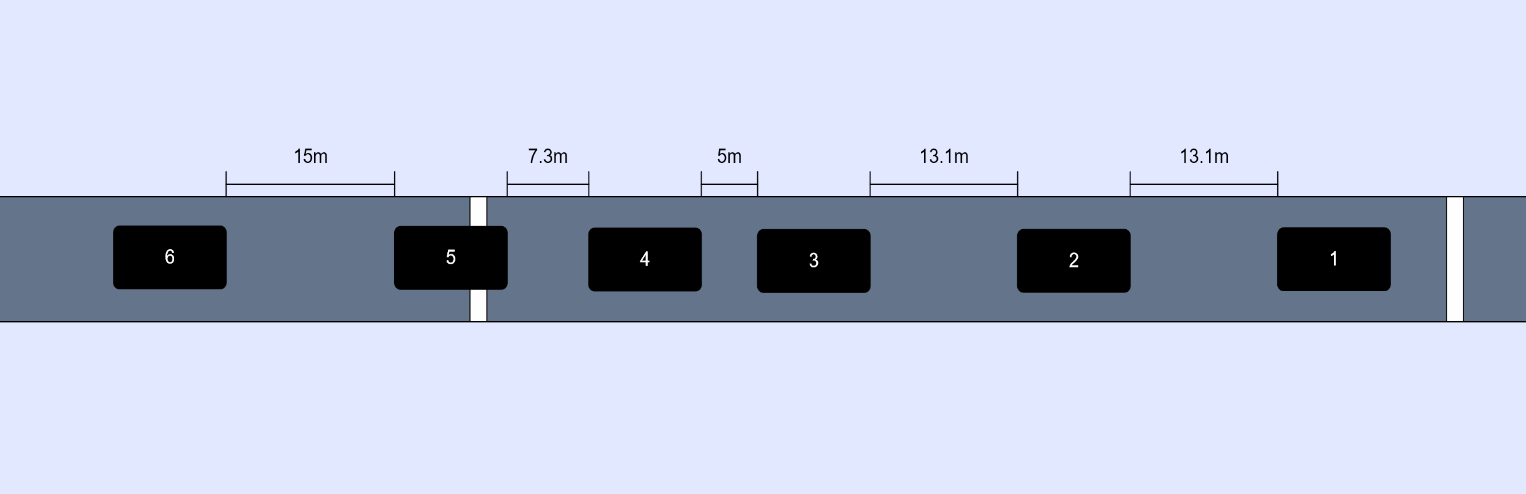
\includegraphics[width=0.85\textwidth, keepaspectratio]{images/3-simulation/simulation-view.png}
    \caption{Visualizzazione grafica della simulazione.}
    \label{fig:simulation-view}
\end{figure}

\newpage
\subsection{Rappresentazione software delle equazioni del platooning}
\begin{tsCode}{Funzione draw() in P5Canvas.tsx}
// Setup for the first car
prevV[0] = velocity[0];
prevU[0] = controlU[0];
acceleration[0] = leadingCarChart[(leadingCarChartIndex + 1) % leadingCarChart.length].velocity - leadingCarChart[leadingCarChartIndex].velocity;
velocity[0] += acceleration[0] / FS;
controlU[0] = acceleration[0];
error[0] = 0;

const standstillDistance = carSpacing * 10 + CAR_WIDTH;

// Update other cars values
for (let i = 1; i < carNumber; i++) {
  // Time i-1 (previous time)
  const prevE = error[i];
  const prevA = acceleration[i];

  // Time i (actual time). Divide Δei, Δvi, Δai, Δui by the simulation frequency 
  error[i] += (prevV[i-1] - prevV[i] - timeHeadway * prevA) / FS;
  velocity[i] += prevA / FS;
  acceleration[i] += ((prevU[i] - prevA) / tau) / FS;
  controlU[i] += ((kp * prevE - kd * prevV[i] - prevU[i] + kd * prevV[i-1] + prevU[i-1]) / timeHeadway - kd * prevA) / FS;

  // di = ei + ri(standstill distace) vi*th(velocity of i vehicle * timeHeadway)
  const desiredDistance = standstillDistance + velocity[i] * timeHeadway;
  let d: number = error[i] + desiredDistance;

  // Limit the distance step & update car positions
  const maxStep = 1;
  const prevDistance = Math.abs(carPoints[i] - carPoints[i-1]);

  if (prevDistance - d > maxStep) {
    d = prevDistance - maxStep;
    for (let j = i; j < carNumber; j++) {
      carPoints[j] += maxStep;
    }
  }
  carPoints[i] = carPoints[i - 1] - d;

  // Update previous velocity & control values
  prevV[i] = velocity[i];
  prevU[i] = controlU[i];
}
\end{tsCode}
\newpage
\section{Frontend}
\fancyhead[RO,LE]{Frontend}

Per sviluppare il progetto abbiamo usato \anchor{\textit{Next.js}}{https://nextjs.org}, framework fullstack per lo sviluppo di applicazioni web, accompagnato da \textit{Typescript} per rendere lo sviluppo più attendibile, aggiungendo sicurezza rispetto ai tipi per tutto il codice.

Tutta la cronologia dello sviluppo è disponibile su \anchor{\textit{Github}}{https://github.com/albbus-stack/platooning-visualization} e la frontend è accessibile pubblicamente su \anchor{platooning-visualization.vercel.app}{https://platooning-visualization.vercel.app}.
Abbiamo optato per ospitare l'app su \anchor{Vercel}{https://vercel.com} dato che offre integrazione/distribuzione continua (\textit{CI}/\textit{CD}), come discuteremo in una sezione successiva.  Il rilascio della nostra applicazione non è tuttavia limitato solo a questa piattaforma ma è anche compatibile con progetti \textit{AWS Amplify} e \textit{Netlify}.

La visualizzazione della simulazione vera e propria è implementata usando \anchor{\textit{P5.js}}{https://p5js.org}, libreria che ci permette di gestire più efficientemente il rendering ad alto frame rate sul \textit{canvas HTML} e che rende disponibile una \textit{API} più ergonomica per interagire con esso.

Per gestire gli stili dell'interfaccia utente abbiamo usato \anchor{\textit{TailwindCSS}}{https://tailwindcss.com}, un framework \textit{CSS} che ci ha permesso di non dividere il codice di rendering dal codice di styling (usando il meccanismo delle classi \textit{CSS}), rendendo lo sviluppo dei componenti \textit{UI} più veloce, rintracciabile e standardizzato.

\begin{tsxCode}{Esempio di classi \textit{TailwindCSS}}
<div className="p-1 text-white transition-all duration-300 rounded-md cursor-pointer select-none bg-slate-800 hover:bg-slate-300 hover:text-slate-800">
      <InfoIcon />
</div>
\end{tsxCode}

Abbiamo reso disponibili anche varie scorciatoie da tastiera per eseguire diverse azioni nell'interfaccia utente, ad esempio \texttt{SPAZIO} mette in pausa o fa partire la simulazione. Nelle sezioni successive ne saranno definite altre in corrispondenza col loro utilizzo.

\newpage
\subsection{Impostazioni}

La gestione dello stato delle impostazioni di simulazione avviene sfruttando il \anchor{\textit{contesto React}}{https://react.dev/learn/passing-data-deeply-with-context}. Il meccanismo di funzionamento del contesto è molto simile a quello del pattern \textit{Provider}/\textit{Consumer} e si divide quindi in due parti:
\vspace{-0.2em}
\begin{itemize}
    \item \textit{Provider}: viene instanziato un componente che racchiude tutti i componenti di cui esso deve gestire lo stato, permettendo interazioni tra loro.\vspace*{-0.5em}
    \item \textit{Consumer}: per consumare (leggere) oppure aggiornare lo stato di un \textit{Provider} viene usato l'\textit{hook} \anchor{\textit{useContext}}{https://react.dev/reference/react/useContext} che espone queste funzionalità ad ogni componente sottostante al \textit{Provider}.
\end{itemize}
\vspace{-0.2em}

Nel nostro caso il \textit{DataProvider} contiene tutte le varie impostazioni della simulazione che possono essere modificate dal componente \textit{DataProvider} (la sezione che contiene i selettori orizzontali per ogni opzione ed il grafico della velocità del primo veicolo); lo stato di queste impostazioni viene in seguito letto dal \textit{canvas P5} per aggiornare la simulazione stessa. Questo meccanismo ci permette quindi di sincronizzare facilmente lo stato tra il componente di modifica e quello di visualizzazione.

Sono disponibili le seguenti impostazioni di simulazione (visibili in figura \ref{fig:simulation-settings}): \textit{Numero di veicoli}, \textit{Distanza obbiettivo tra di loro}, \textit{Distanza temporale tra di loro}, \textit{Delay di comunicazione} ed alcuni parametri del modello di platooning precedentemente discusso come \textit{Tau}, \textit{Kp} e \textit{Kd}.

\begin{figure}[H]
    \vspace{0.7em}
    \centering
    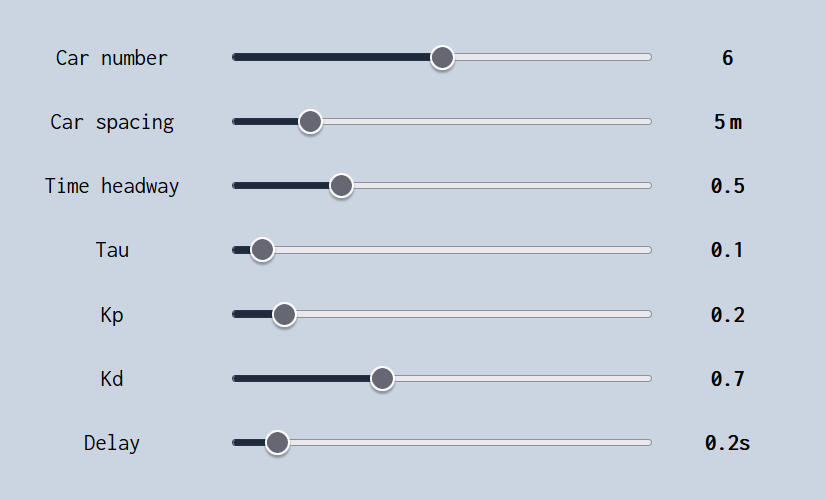
\includegraphics[width=0.75\textwidth, keepaspectratio]{images/4-frontend/simulation-settings.png}
    \caption{Varie impostazioni numeriche per la simulazione.}
    \label{fig:simulation-settings}
\end{figure}

\begin{figure}[H]
    \vspace{0.5em}
    \centering
    \captionsetup{justification=centering, margin=2cm}
    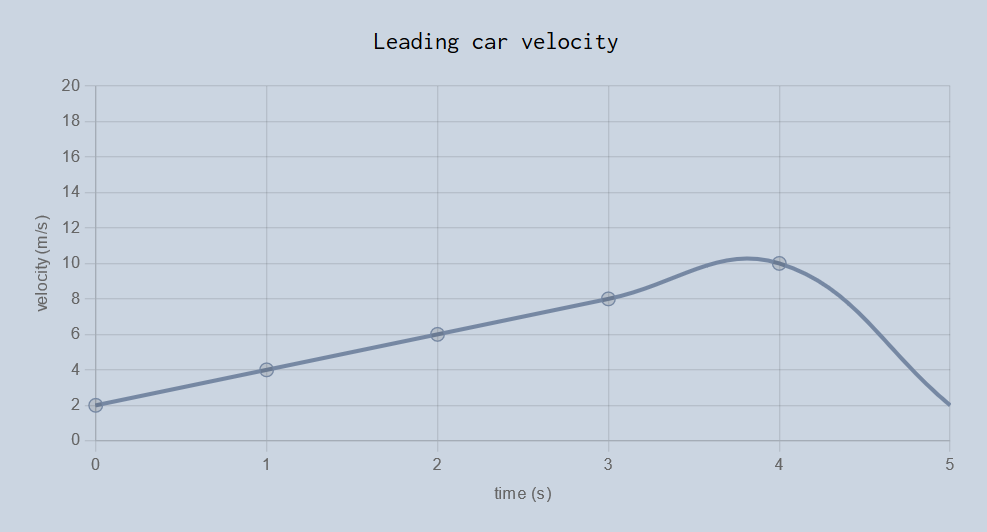
\includegraphics[width=0.75\textwidth, keepaspectratio]{images/4-frontend/velocity-settings.png}
    \caption{Grafico per impostare l'andamento del primo veicolo del convoglio nel tempo.}
    \label{fig:velocity-settings}
\end{figure}

\begin{figure}[H]
    \centering
    \captionsetup{justification=centering, margin=2cm}
    
\includegraphics[width=0.65\textwidth, keepaspectratio]{images/4-frontend/keyboard-shortcuts.png}
    \caption{Interfaccia utente per l'apertura dei pannelli (\textit{Sliver}), con sopra annotate le scorciatoie da tastiera.}
    \label{fig:keyboard-shortcuts}
\end{figure}

La velocità del primo veicolo del convoglio è controllabile tramite un grafico interattivo, in figura \ref{fig:velocity-settings}, in cui sono modificabili i punti da $t=0$ a $t=4$. Il primo veicolo segue in maniera periodica questo grafico delle velocità con accelerazione uniforme. Come descritto nella sezione successiva, è stato scelto \textit{ChartJS} per produrre anche questo grafico interattivo.

Le impostazioni per la simulazione ed i grafici risultanti sono contenute in due pannelli separati, accessibili tramite due bottoni nell'interfaccia utente (visibili in figura \ref{fig:keyboard-shortcuts}) oppure usando delle scorciatoie da tastiera: \texttt{G} per aprire il pannello dei grafici (\textit{GraphSliver}) e \texttt{S} per aprire il pannello delle impostazioni (\textit{SettingSliver}).

Dopo aver configurato i parametri desiderati, è possibile avviare la simulazione per visualizzare il comportamento del veicolo in base alle scelte effettuate. L'uso di grafici e impostazioni personalizzabili permette un'analisi interattiva del modello di platooning da parte dell'utente.

\newpage
\subsubsection*{Codice allegato}

\vspace{0.3em}
\begin{tsCode}{Gestione dello stato delle impostazioni con \textit{DataProvider}}
/* DataProvider.tsx */
export const DataProvider: React.FC<DataProviderProps> = ({ children }) => {
  const [carNumber, setCarNumber] = useState(6);
  const [carSpacing, setCarSpacing] = useState(5.0);
  const [timeHeadway, setTimeHeadway] = useState(0.5);
  const [tau, setTau] = useState(0.1);
  const [kp, setKp] = useState(0.2);
  const [kd, setKd] = useState(0.7);
  const [velocityFrameDelay, setVelocityFrameDelay] = useState(VELOCITY_DELAY);
  const [leadingCarChart, setLeadingCarChart] = useState<GraphPoints[]>(
    [0, 1, 2, 3, 4].map((i) => {
      return {
        time: i,
        velocity: i * 2 + 2,
      };
    })
  );
  ...
}

/* SettingsSliver.tsx */
const SettingsSliver: React.FC = () => {
  const { carNumber, setCarNumber, carSpacing, setCarSpacing, ... } = useContext(DataContext);
  ...
}

/* P5Canvas.tsx */
<NextReactP5Wrapper
  sketch={sketch}
  carSpacing={carSpacingSetting}
  carNumber={carNumberSetting}
  ...
>
\end{tsCode}
\vspace{0.6em}

Le varie impostazioni della simulazione sono contenute dentro \textit{DataProvider} e i loro stati sono inizializzati con dei valori di default, inclusi i punti del grafico della velocità del primo veicolo. In seguito \textit{SettingSliver} utilizza i \textit{getter} e \textit{setter} esposti da questo provider per permettere all'utente di modificare le impostazioni interattivamente attraverso gli slider.

Infine nel \textit{canvas P5} viene letto lo stato del contesto e passato all'istanza sottostante di \textit{P5.js} attraverso i \textit{props} del componente \textit{NextReactP5Wrapper} che rende la simulazione consapevole del cambiamento di qualsiasi di questi, in maniera reattiva.

\newpage
\subsection{Grafici}

La visualizzazione dei grafici è implementata usando \anchor{\textit{ChartJS}}{https://www.chartjs.org}, libreria molto popolare grazie alla performance del \textit{canvas HTML} e alla sua interazione stretta con \textit{React} (attraverso la libreria wrapper \anchor{\textit{react-chartjs-2}}{https://react-chartjs-2.js.org}).

Come suggerito precedentemente, la gestione dei dati usati per la produzione dei grafici è sempre affidata al \textit{contesto React}, in particolare al componente \textit{DataProvider} che espone \textit{getter} e \textit{setter} relativi ai dati di distanza e velocità tra i veicoli. Questo approccio ci consente di gestire in modo efficiente e organizzato tutti i dati relativi alla simulazione, garantendo una facile integrazione con il resto dell'applicazione.

La simulazione \textit{P5} stessa esegue a \textit{60 fps} e viene campionata ogni quarto di secondo ($250ms$) per raccogliere questi dati di distanza e velocità. Quando viene aggiunto un nuovo \textit{DataPoint}, i grafici contenuti in \textit{GraphSliver} si aggiornano, mostrando dinamicamente i dati raccolti, permettendo quindi agli utenti di monitorare l'evoluzione della simulazione in tempo reale. 

Nell'interfaccia utente è possibile visualizzare il grafico di distanza o velocità specifico per un veicolo; questi sono selezionabili da due dropdown presenti sopra ai grafici corrispondenti. 

E' possibile osservare un esempio della visualizzazione di questa sezione in figura \ref{fig:distance-graph} e \ref{fig:velocity-graph}.

\begin{figure}[H]
    \vspace{1em}
    \centering
    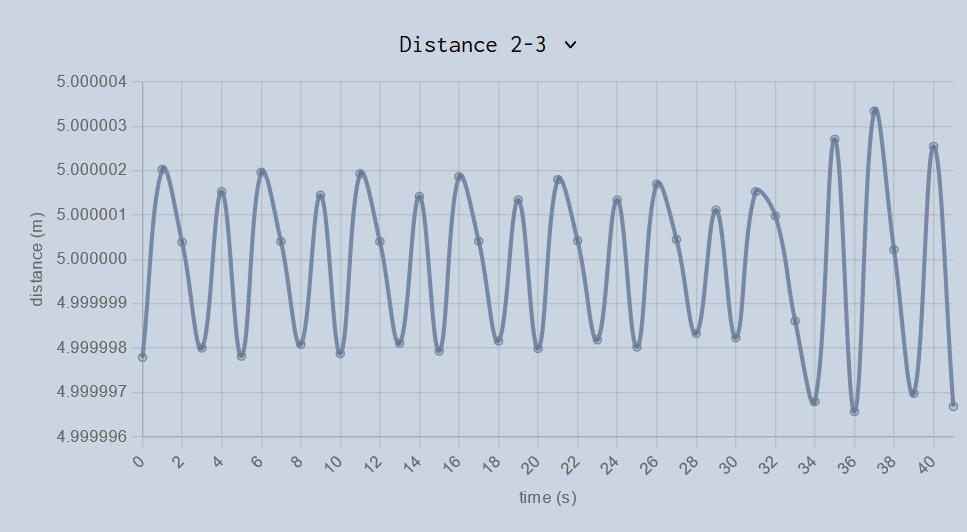
\includegraphics[width=0.85\textwidth, keepaspectratio]{images/4-frontend/distance-graph.png}
    \caption{Grafico della distanza tra due veicoli del convoglio.}
    \label{fig:distance-graph}
\end{figure}

\begin{figure}[H]
    \vspace{0.5em}
    \centering
    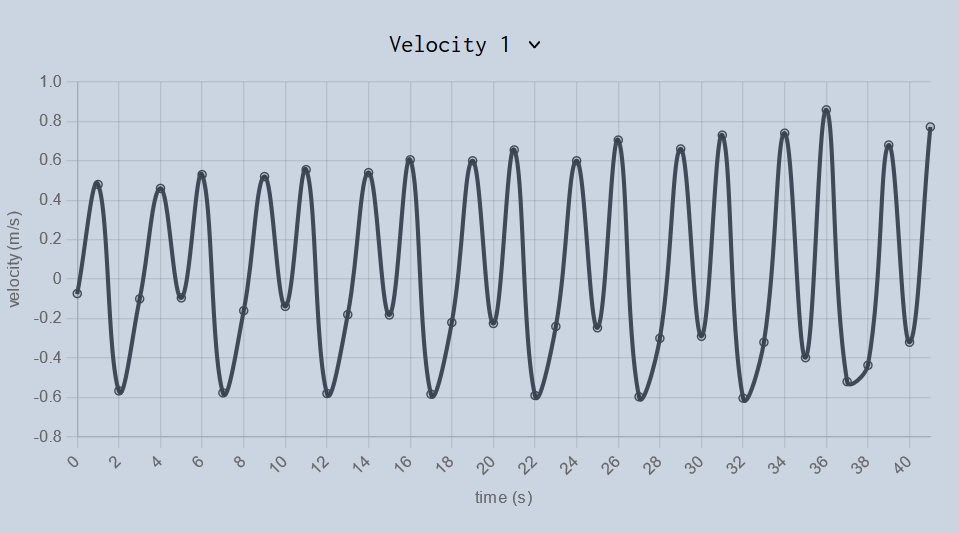
\includegraphics[width=0.85\textwidth, keepaspectratio]{images/4-frontend/velocity-graph.png}
    \caption{Grafico della velocità di un veicolo del convoglio.}
    \label{fig:velocity-graph}
\end{figure}

\begin{figure}[H]
    \centering
    \captionsetup{justification=centering, margin=3cm}
    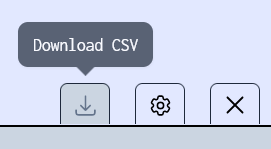
\includegraphics[width=0.55\textwidth, keepaspectratio]{images/4-frontend/csv-export.png}
    \caption{Bottone di esportazione dei dati della simulazione in \texttt{csv}.}
    \label{fig:csv-export}
\end{figure}

Un aspetto utile della nostra implementazione è la possibilità di esportare i dati raccolti in formato \texttt{csv} con la seguente struttura: \texttt{carNumber}, \texttt{time(s)}, \texttt{distance(m)}, \texttt{velocity(m/s)}. Dove \texttt{time(s)} è l'istante di tempo e \texttt{distance} si riferisce alla distanza tra il veicolo \texttt{carNumber} e \texttt{carNumber+1}. Per l'ultimo veicolo questa distanza sarà sempre considerata 0 come default dato che non c'è nessun veicolo successivo ad esso.

Il download in formato \texttt{csv} consente agli utenti di analizzare i dati della simulazione in dettaglio al di fuori dell'applicazione, utilizzando strumenti esterni o elaborando i risultati in altri contesti. In figura \ref{fig:csv-export} è visibile l'interfaccia utente per questa funzione.

\newpage
\subsubsection*{Codice allegato}

\vspace{0.3em}
\begin{tsCode}{Gestione dello stato dei grafici con \textit{DataProvider}}
/* DataProvider.tsx */
export const DataProvider: React.FC<DataProviderProps> = ({ children }) => {
  const [graphData, setGraphData] = useState([[]] as {
    distance: number;
    velocity: number;
    time: number;
  }[][]);
  ...
}

/* GraphSliver.tsx */
const GraphSliver: React.FC = () => {
  const [distanceChartIndex, setDistanceChartIndex] = useState(0);
  const [velocityChartIndex, setVelocityChartIndex] = useState(0);

  const { graphData } = useContext(DataContext);
  ...
}

/* P5Canvas.tsx */
const { setGraphData } = useContext(DataContext);

intervalRef = setInterval(() => {
  timeTick++;
  setGraphData((car) => 
    car.map((prev, i) => [ 
      ...prev, 
      { time: timeTick, distance: distance[i], velocity: velocity[i] },
    ])
  );
}, UPDATE_INTERVAL);
\end{tsCode}
\vspace{0.6em}

Come si può osservare sopra, \textit{DataProvider} contiene i dati di distanza e velocità di ogni veicolo per ogni istante di tempo. Questo stato è letto da \textit{GraphSliver} che ha due variabili di stato locali contenenti gli indici dei grafici di distanza e velocità attualmente selezionati dall'utente nella sezione corrispondente.

Lo stato del \textit{DataProvider} viene aggiornato dentro un \textit{intervallo} (cioè una \textit{API} per ripetere l'esecuzione di un blocco di codice periodicamente) nel \textit{canvas P5} che contiene i dati della simulazione in esecuzione. Nel nostro caso l'intervallo esegue ogni \texttt{UPDATE\_INTERVAL} millisecondi, costante definita precedentemente nel file ad un secondo; per ottenere dati in uscita con frequenza di campionamento più alta è sufficiente modificare questo valore.

\newpage
\subsection{Scorciatoie da tastiera}

Abbiamo aggiunto varie scorciatoie da tastiera per interagire con l'interfaccia utente più rapidamente. Segue un elenco di alcuni di questi \textit{shortcuts}: 
\begin{itemize}
\setlength{\itemsep}{-0.1em}
    \item \texttt{SPAZIO} avvia o interrompe la simulazione.
    \item \texttt{R} ripristina la simulazione alle impostazioni predefinite.
    \item \texttt{S} apre la sezione per la modifica delle impostazioni (\textit{SettingsSliver}).
    \item \texttt{G} apre la sezione di visualizzazione dei grafici (\textit{GraphSliver}).
    \item \texttt{D} scarica i dati in \texttt{csv} della simulazione eseguita.
    \item \texttt{$\uparrow$} e \texttt{$\downarrow$} ingrandiscono/diminuiscono la dimensione della \textit{Sliver}.
    \item \texttt{$\leftarrow$} e \texttt{$\rightarrow$} ciclano tra \textit{Sliver} delle impostazioni e dei grafici.
    \item \texttt{ESC} chiude la \textit{Sliver}.
\end{itemize}

\subsubsection*{Codice allegato}
\vspace{0.1em}
\begin{tsCode}{Gestione delle scorciatoie da tastiera in \textit{P5Canvas.tsx}}
useEffect(() => {  
  const onKeyDown = (e: KeyboardEvent) => {
     switch (e.key) {
      // Start/stop the simulation
      case " ":
        togglePlay();
        break;

      // Reset the simulation 
      case "r":
        resetCanvas(window.innerWidth, carNumberSetting, carSpacingSetting);
        break;
      ...
    }
  }

  document.addEventListener("keydown", onKeyDown);
  return () => document.removeEventListener("keydown", onKeyDown);
}, [togglePlay])
\end{tsCode}

% /* Sliver.tsx */
% const onKeyDown = (e: KeyboardEvent) => {
%   switch (e.key) {
%     // Download the graph data
%     case "d":
%       if (isGraphSliver && isSliverOpen) {
%         downloadGraphDataCSV(graphData);
%       }
%       break;

%     // Close the sliver
%     case "Escape":
%       setIsSliverOpen(false);
%       break;
%     ...
%   }
% }
\vspace{0.3em}

Il codice fornito gestisce le scorciatoie per \texttt{SPAZIO} e \texttt{R} utilizzando \textit{useEffect}. Con questo hook viene registrato un gestore per gli eventi \textit{keydown} quando il componente viene montato. Questo gestore di eventi controlla quale tasto è stato premuto attraverso l'oggetto \textit{KeyboardEvent} e reagisce di conseguenza. Oltre a questo \textit{useEffect} ritorna una funzione di \textit{cleanup} dove viene rilasciato il gestore delle scorciatoie.

\newpage
\subsection{Internazionalizzazione}

Per rendere questo progetto fruibile da utenti che non parlano l'inglese abbiamo deciso di implementare un sistema di internazionalizzazione che include le seguenti localizzazioni: \textit{en}, \textit{it}, \textit{fr}, \textit{es}, \textit{de}, \textit{dk}, \textit{nl}, \textit{pt}, \textit{ru}, \textit{sa}, \textit{in}, \textit{cn}, \textit{jp}, \textit{kr}.
 
Questa funzionalità è stata raggiunta usando le \anchor{\textit{Dynamic Routes}}{https://nextjs.org/docs/pages/building-your-application/routing/dynamic-routes}; queste consistono nel raccogliere il codice di rendering per varie \textit{routes} (percorsi del sito) dentro un solo componente.   
Nel nostro caso ci permettono di cambiare il linguaggio selezionato semplicemente rimandando al percorso "\texttt{/locale}" corrispondente (dove \texttt{locale} è una delle stringhe di localizzazione sopra elencate).
Per la lingua di default, cioè l'inglese, il percorso usato è "\texttt{/}" senza nessuna specificazione di lingua ulteriore, come vediamo in figura \ref{fig:dynamic-routes}.

La gestione vera e propria delle varie traduzioni è stata affidata a \anchor{\textit{ParaglideJS}}{https://inlang.com/m/gerre34r/library-inlang-paraglideJs}, un nuovo e promettente framework di internazionalizzazione. Questa libreria gestisce lo stato locale del client riguardante la lingua attualmente selezionata ed espone una semplice \textit{API} per leggerlo e modificarlo, tutto mantenendo completamente la \textit{type safety}.

Le stringhe di traduzione sono scritte in dei file \texttt{json} e possiamo aggiungere altre lingue semplicemente scrivendone uno nuovo e ricompilando il \textit{bundle} di \textit{ParaglideJS} (affinché tutte le stringhe siano controllate ed esportate staticamente prima della build del progetto).    

Per mostrare le bandiere corrispondenti ad ognuna delle lingue utilizzate abbiamo usato degli \texttt{svg} resi disponibili dalla repository \anchor{\textit{country-flags}}{https://github.com/hampusborgos/country-flags/tree/main/svg}.

\begin{figure}[H]
    \vspace{0.8em}
    \centering
    \captionsetup{justification=centering, margin=1.5cm}
    
\includegraphics[width=0.7\textwidth, keepaspectratio]{images/4-frontend/dynamic-routes.png}
    \caption{Percorsi dinamici corrispondenti ad inglese (\texttt{/}), italiano (\texttt{/it}) e francese (\texttt{/fr}).}
    \label{fig:dynamic-routes}
\end{figure}

\newpage
\subsubsection*{Codice allegato}

\vspace{0.2em}
\begin{tsCode}{Utilizzo di \textit{ParaglideJS} per l'internazionalizzazione}
/* pages/[locale]/index.tsx */
import { AvailableLanguageTag, availableLanguageTags, setLanguageTag } from "../../src/paraglide/runtime";
import { useRouter } from "next/router";

const Home: NextPage = () => {
  const router = useRouter();
  const locale = router.query.locale as AvailableLanguageTag ?? "en";

  if (availableLanguageTags.includes(locale)) {
    setLanguageTag(locale);
  } else if (router.query.locale) {
    return <PageNotFound />;
  }

  return <HomePage />;
};

/* translations/it.json */
{
  "$schema": "https://inlang.com/schema/inlang-message-format",
  "title": "Simulazione di platooning",
  "graphs": "Grafici",
  "settings": "Impostazioni", ...
}

/* package.json */
{
  "name": "platooning-visualization",
  "scripts": {
    "lang": "paraglide-js compile --project ./project.inlang.json",
  }, ...
}
\end{tsCode}
\vspace{0.4em}

Come si può osservare, i percorsi dinamici sono gestiti attraverso l'\textit{hook} \anchor{\textit{useRouter}}{https://nextjs.org/docs/pages/api-reference/functions/use-router} che raccoglie la stringa corrispondente alla \textit{route} visitata nell'attributo \texttt{query.locale}. Se viene fornita una stringa vuota il \textit{type cast} la assegnerà al valore della \textit{locale} di default (\texttt{"en"}), altrimenti se viene fornita una stringa di localizzazione non valida verrà renderizzata una \textit{pagina 404} (pagina non trovata; contenente un link alla pagina principale).

Come discusso in precedenza le stringhe delle traduzioni sono contenute in dei file \texttt{json} e dobbiamo compilare i messaggi di \textit{ParaglideJS} ogni volta che queste vengono aggiornate (attraverso lo script eseguibile con \texttt{pnpm lang}).

\newpage
\subsection{Integrazione Continua}

Per garantire un flusso di sviluppo fluido e automatizzato, abbiamo configurato un sistema di integrazione continua utilizzando \textit{Vercel} e \anchor{la loro integrazione \textit{GitHub}}{https://vercel.com/docs/deployments/git/vercel-for-github}.

\textit{Vercel}, una piattaforma di hosting specializzata nel \textit{deploy} di applicazioni \textit{React} e \textit{Next.js}, offre un'integrazione continua semplice ed efficace: ogni volta che viene eseguito un commit o viene aperta una pull request sul branch principale della nostra repository viene avviato automaticamente un processo di build e distribuzione dell'applicazione.

Questo processo assicura che ogni modifica apportata al codice venga immediatamente testata e poi resa disponibile. Inoltre, \textit{Vercel} offre la funzionalità dei \textit{deployment} di preview, con la possibilità di creare anteprime delle modifiche non ancora pubblicate al pubblico, consentendo un controllo prima che queste vengano distribuite ufficialmente.

\vspace{-0.4em}
\subsubsection*{Codice allegato}

\vspace{0.3em}
\begin{tsCode}{Integrazione continua con \textit{Vercel}}
/* package.json */
{
  "name": "platooning-visualization",
  "scripts": {
    "lint": "next lint",
    "build": "pnpm lint && pnpm lang && pnpm next build",
  }, ...
}
\end{tsCode}
\vspace{0.3em}

Questo \textit{snippet} indica come vengono gestiti i passaggi di build dell'applicazione durante il processo di integrazione continua:

\vspace{-0.4em}
\begin{itemize}
\setlength{\itemsep}{-0.1em}
    \item \texttt{pnpm lint}: prima di avviare il processo di build, viene eseguito il comando di \textit{linting} per assicurarsi che il codice sia conforme agli standard definiti.
    \item \texttt{pnpm lang}: vengono poi compilate le traduzioni dell'applicazione per renderle disponibili al runtime di \textit{ParaglideJS} come discusso in precedenza.
    \item \texttt{pnpm next build}: infine viene avviato il processo di build ed esportazione dell'applicazione utilizzando \textit{Next.js}.
\end{itemize}
\newpage
\section{Esperimenti}
\fancyhead[RO,LE]{Esperimenti}

I grafici sottostanti sono stati generati con uno script \textit{Python} a partire da dei \texttt{.csv} esportati dall'interfaccia web, tutte queste risorse sono disponibili nella cartella \texttt{experiments} sulla \anchor{repository \textit{Github}}{https://github.com/albbus-stack/platooning-visualization/tree/main/experiments} divise in cartelle relative al parametro testato.

\begin{pyCode}{Generazione dei grafici con \textit{Matplotlib}}
def plot_and_save(output_filename, data, ylabel):
  for car_index, car_data in data.items():
    if ylabel == 'distance' and car_index == len(data.items()) - 1:
      continue
    plt.plot(car_data['time'], car_data[ylabel], marker='o', linestyle='-', 
      label=f'Auto {car_index + 1}' if ylabel == 'velocity'
        else f'Distanza {car_index + 1}-{car_index + 2}')

  plt.xlabel('Tempo (s)')
  plt.ylabel('Velocità (m/s)' if ylabel == 'velocity' else 'Distanza (m)')
  plt.legend()
  plt.savefig(output_filename)
  plt.close()
\end{pyCode}

\newpage
\subsection{Modello stabile}

% DEFAULT %

\subsubsection{Parametri di default}
Questi parametri sono presi dall'articolo \cite{ploeg_2014_lp}.

%\begin{table}[h]
%    \centering
%    \begin{tabular}{|c|c|c|c|c|}
%        \hline
%        Velocità $t1$ & Velocità $t2$ & Velocità $t3$ &Velocità $t4$ &Velocità $t5$\\
%        \hline
%            $2\hspace{0.2em}m/s$ & $4\hspace{0.2em}m/s$ & $6\hspace{0.2em}m/s$ & $8\hspace{0.2em}m/s$ & $10\hspace{0.2em}m/s$ \\
%        \hline
%    \end{tabular}
%    \label{tab:experiment_velocities}
%\end{table}
\begin{table}[h]
    \centering
    \begin{tabular}{|c|c|c|c|}
        \hline
        N° auto & Distanza Iniziale & Distanza Target & Ritardo \\
        \hline
        $6$ & $6.0 m$ & $5.0 m$ & $0.2 s$ \\
        \hline
        $Time\hspace{0.2em}Headway$ & $\tau$ & $K_p$ & $K_d$  \\
        \hline
        $0.5$ & $0.1$ & $0.2$ & $0.7$ \\
        \hline
    \end{tabular}
    \label{tab:default_parameters}
\end{table}

\begin{figure}[H]
    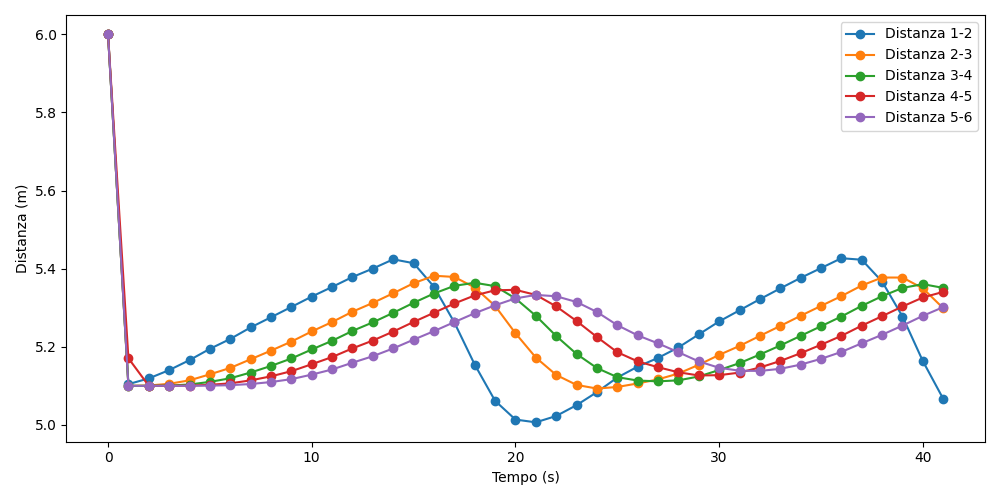
\includegraphics[width=0.96\textwidth]{images/5-experiment/default/distance_6.png}
    \caption{Distanze con parametri di default.}
    \label{fig:default-distance}
\end{figure}

\begin{figure}[H]
    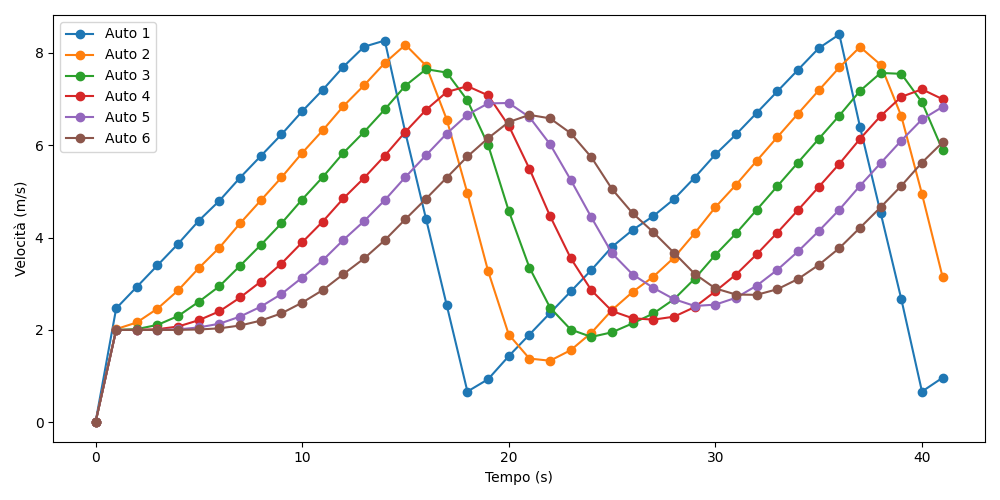
\includegraphics[width=0.96\textwidth]{images/5-experiment/default/velocity_6.png}
    \caption{Velocità con parametri di default.}
    \label{fig:default-velocity}
\end{figure}
\newpage

% CAR NUMBER %

\subsubsection{Numero di auto}
\vspace*{\fill}
\begin{table}[h]
    \centering
    \begin{tabular}{|c|c|c|c|}
        \hline
        N° auto & Distanza Iniziale & Distanza Target & Ritardo \\
        \hline
        $3$ & $6.0 m$ & $5.0 m$ & $0.2 s$ \\
        \hline
        $Time\hspace{0.2em}Headway$ & $\tau$ & $K_p$ & $K_d$  \\
        \hline
        $0.5$ & $0.1$ & $0.2$ & $0.7$ \\
        \hline
    \end{tabular}
\end{table}

\begin{figure}[H]
    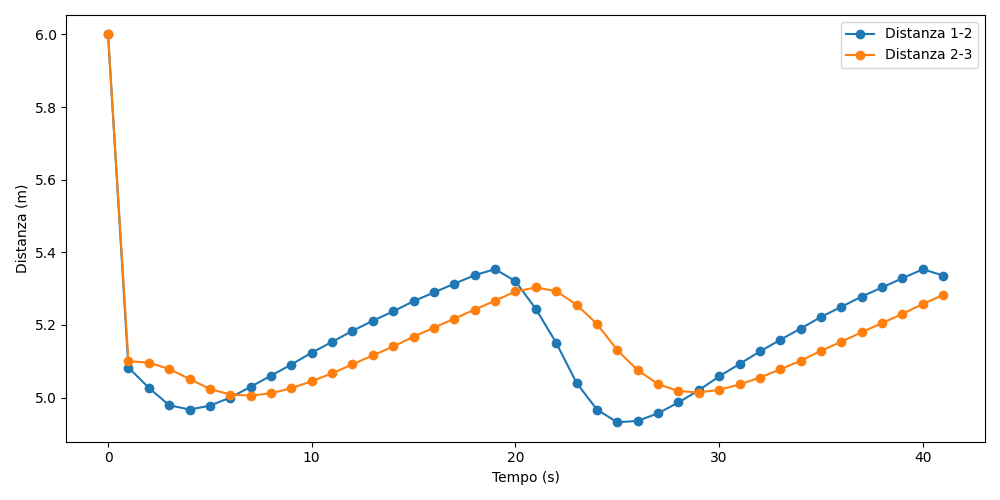
\includegraphics[width=0.96\textwidth]{images/5-experiment/car-number/distance_3.png}
    \caption{Distanze con 3 auto.}
    \label{fig:3-cars-distance}
\end{figure}

\begin{figure}[H]
    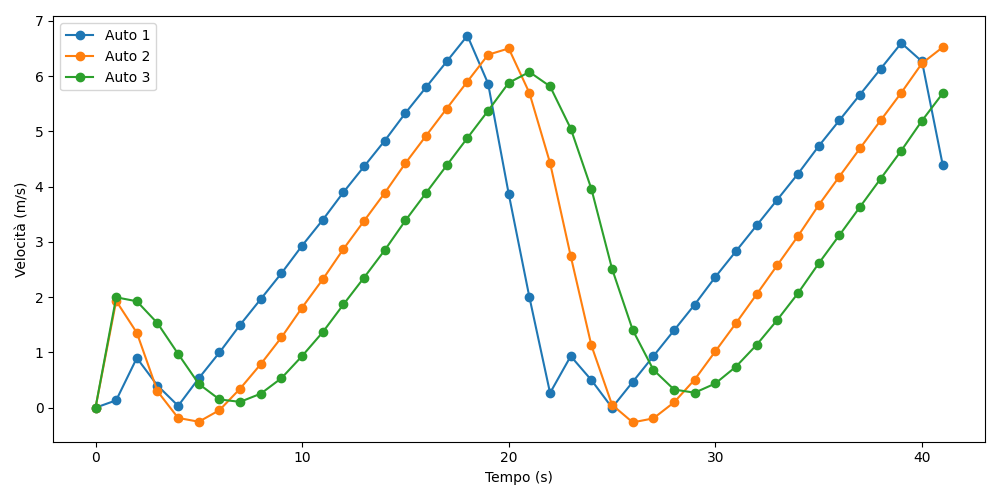
\includegraphics[width=0.96\textwidth]{images/5-experiment/car-number/velocity_3.png}
    \caption{Velocità con 3 auto.}
    \label{fig:3-cars-velocity}
\end{figure}
\vspace*{\fill}
\newpage
\vspace*{\fill}
\begin{table}[h]
    \centering
    \begin{tabular}{|c|c|c|c|}
        \hline
        N° auto & Distanza Iniziale & Distanza Target & Ritardo \\
        \hline
        $8$ & $6.0 m$ & $5.0 m$ & $0.2 s$ \\
        \hline
        $Time\hspace{0.2em}Headway$ & $\tau$ & $K_p$ & $K_d$  \\
        \hline
        $0.5$ & $0.1$ & $0.2$ & $0.7$ \\
        \hline
    \end{tabular}
\end{table}

\begin{figure}[H]
    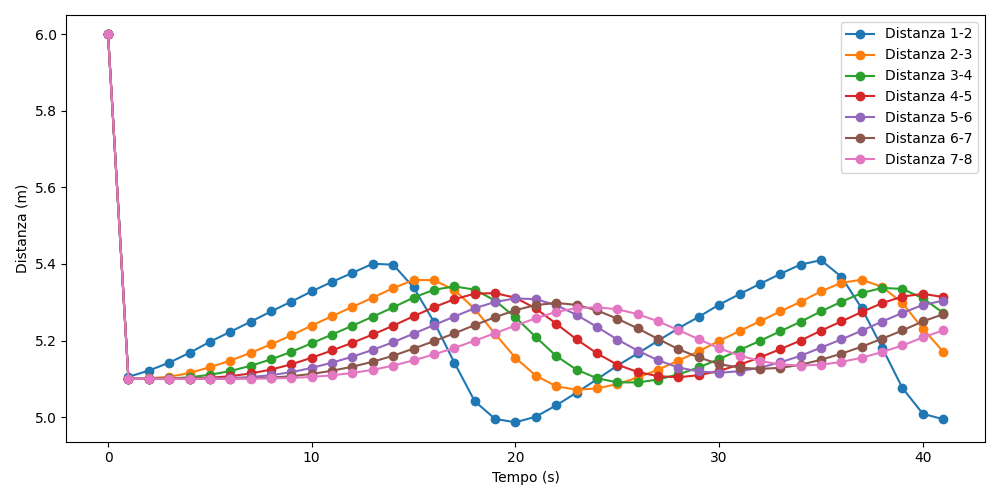
\includegraphics[width=0.96\textwidth]{images/5-experiment/car-number/distance_8.png}
    \caption{Distanze con 8 auto.}
    \label{fig:8-cars-distance}
\end{figure}

\begin{figure}[H]
    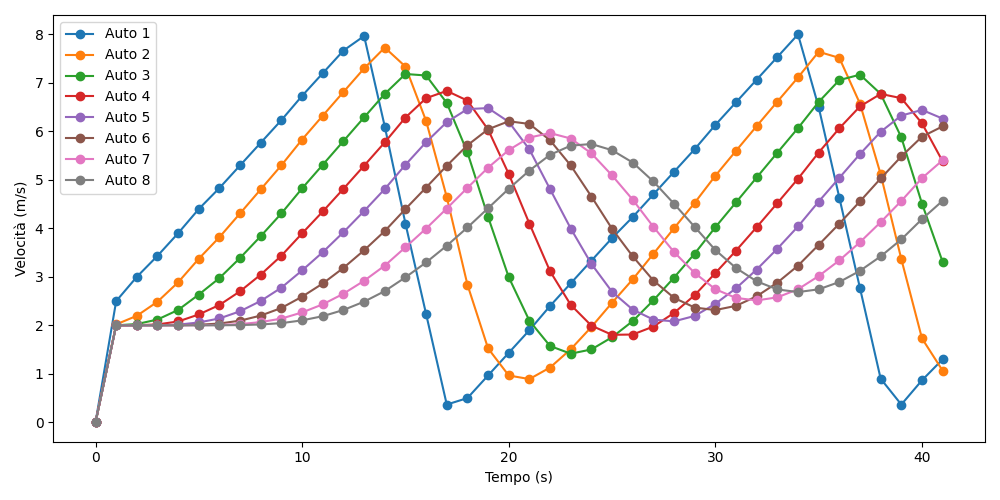
\includegraphics[width=0.96\textwidth]{images/5-experiment/car-number/velocity_8.png}
    \caption{Velocità con 8 auto.}
    \label{fig:8-cars-velocity}
\end{figure}
\vspace*{\fill}
\newpage
\vspace*{\fill}
\begin{table}[h]
    \centering
    \begin{tabular}{|c|c|c|c|}
        \hline
        N° auto & Distanza Iniziale & Distanza Target & Ritardo \\
        \hline
        $10$ & $6.0 m$ & $5.0 m$ & $0.2 s$ \\
        \hline
        $Time\hspace{0.2em}Headway$ & $\tau$ & $K_p$ & $K_d$  \\
        \hline
        $0.5$ & $0.1$ & $0.2$ & $0.7$ \\
        \hline
    \end{tabular}
\end{table}

\begin{figure}[H]
    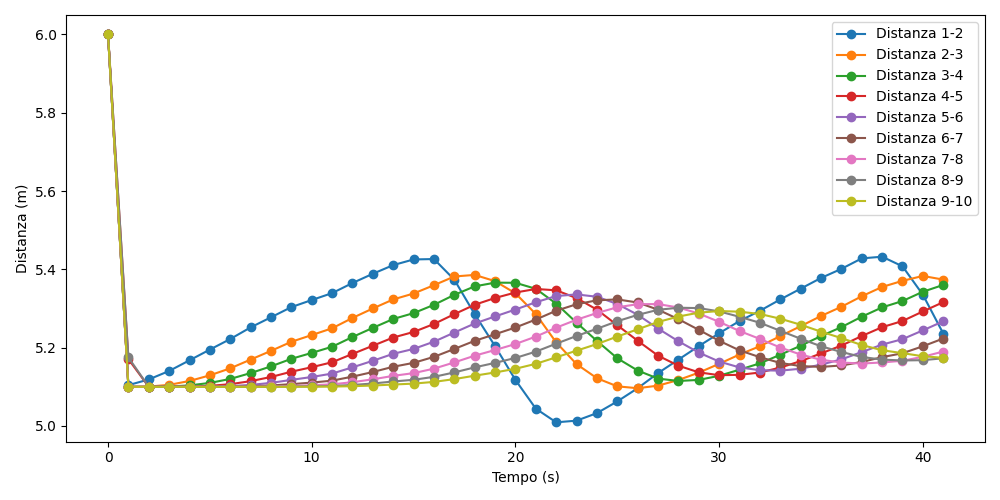
\includegraphics[width=0.96\textwidth]{images/5-experiment/car-number/distance_10.png}
    \caption{Distanze con 10 auto.}
    \label{fig:10-cars-distance}
\end{figure}

\begin{figure}[H]
    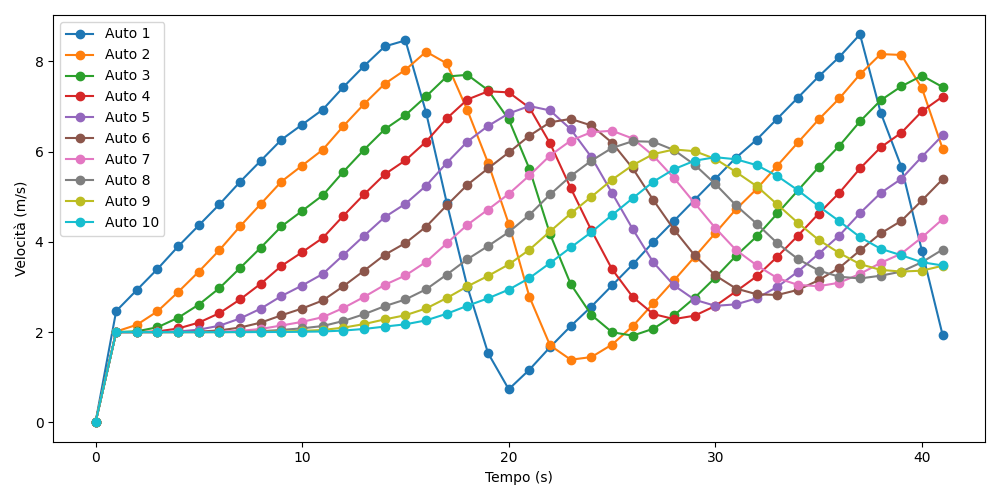
\includegraphics[width=0.96\textwidth]{images/5-experiment/car-number/velocity_10.png}
    \caption{Velocità con 10 auto.}
    \label{fig:10-cars-velocity}
\end{figure}

\vspace*{\fill}
\newpage

% CAR SPACING %

\subsubsection{Spazio tra le auto}
\vspace*{\fill}
\begin{table}[h]
    \centering
    \begin{tabular}{|c|c|c|c|}
        \hline
        N° auto & Distanza Iniziale & Distanza Target & Ritardo \\
        \hline
        $6$ & $2.0 m$ & $5.0 m$ & $0.2 s$ \\
        \hline
        $Time\hspace{0.2em}Headway$ & $\tau$ & $K_p$ & $K_d$  \\
        \hline
        $0.5$ & $0.1$ & $0.2$ & $0.7$ \\
        \hline
    \end{tabular}
\end{table}

\begin{figure}[H]
    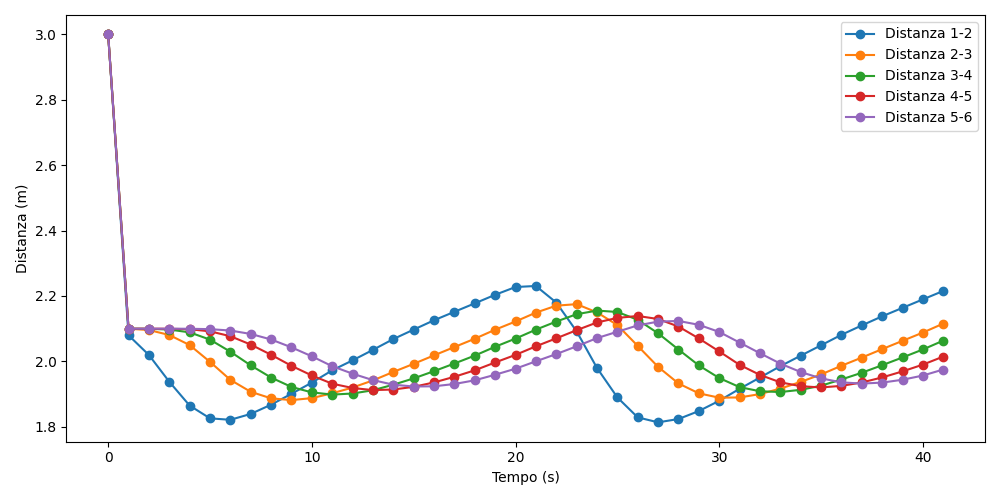
\includegraphics[width=0.96\textwidth]{images/5-experiment/car-spacing/distance_2.png}
    \caption{Distanze con $2.0 m$ come distanza iniziale.}
    \label{fig:2-space-distance}
\end{figure}

\begin{figure}[H]
    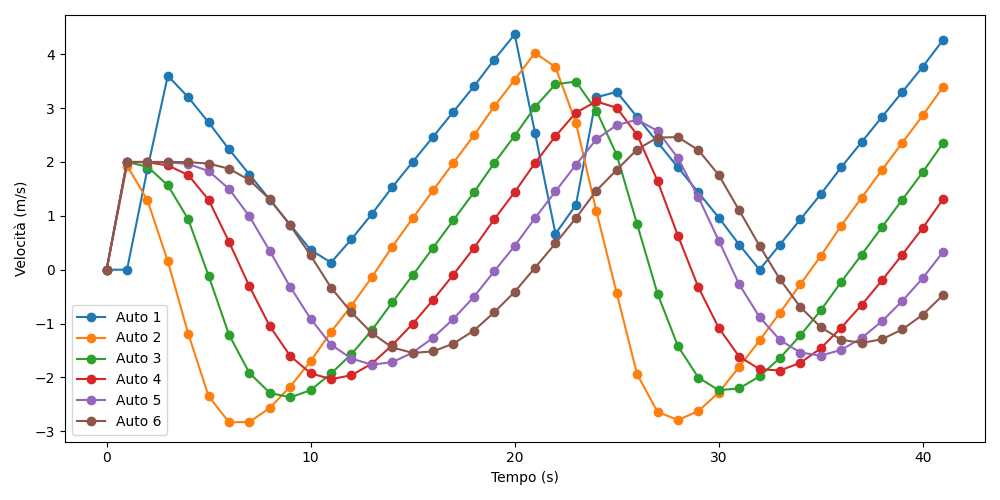
\includegraphics[width=0.96\textwidth]{images/5-experiment/car-spacing/velocity_2.png}
    \caption{Velocità con distanza iniziale $2.0 m$.}
    \label{fig:2-space-velocity}
\end{figure}
\vspace*{\fill}
\newpage
\vspace*{\fill}
\begin{table}[h]
    \centering
    \begin{tabular}{|c|c|c|c|}
        \hline
        N° auto & Distanza Iniziale & Distanza Target & Ritardo \\
        \hline
        $6$ & $10.0 m$ & $5.0 m$ & $0.2 s$ \\
        \hline
        $Time\hspace{0.2em}Headway$ & $\tau$ & $K_p$ & $K_d$  \\
        \hline
        $0.5$ & $0.1$ & $0.2$ & $0.7$ \\
        \hline
    \end{tabular}
\end{table}
\begin{figure}[H]
    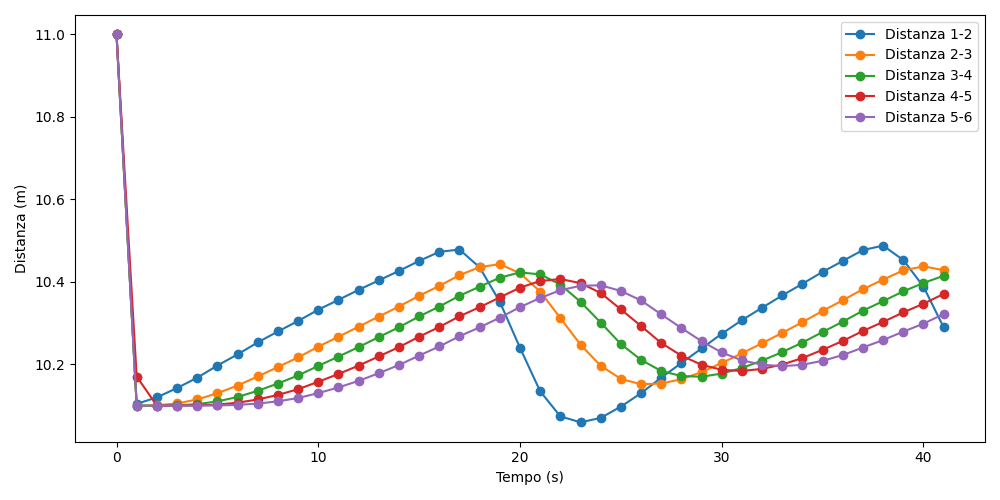
\includegraphics[width=0.96\textwidth]{images/5-experiment/car-spacing/distance_10.png}
    \caption{Distanze con $10.0 m$ come distanza iniziale.}
    \label{fig:10-space-distance}
\end{figure}

\begin{figure}[H]
    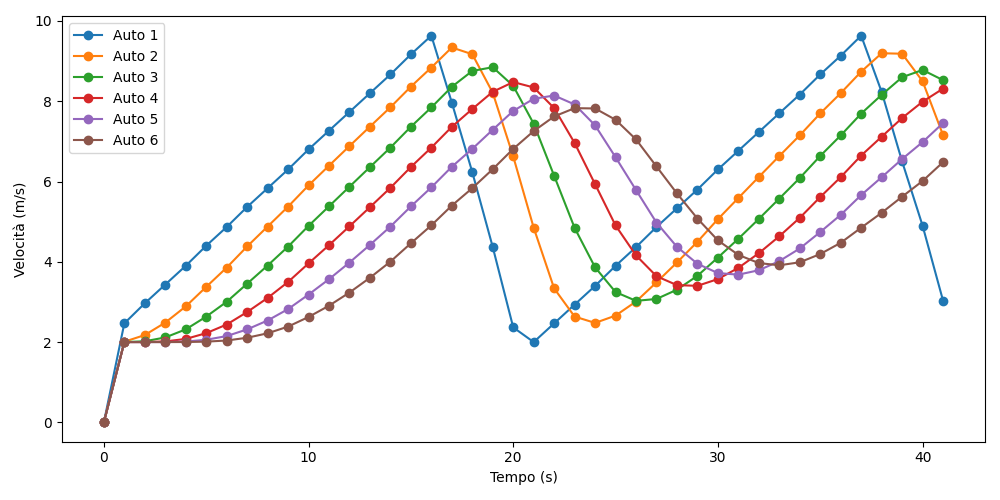
\includegraphics[width=0.96\textwidth]{images/5-experiment/car-spacing/velocity_10.png}
    \caption{Velocità con distanza iniziale $10.0 m$.}
    \label{fig:10-space-velocity}
\end{figure}
\vspace*{\fill}
\newpage
\vspace*{\fill}
\begin{table}[h]
    \centering
    \begin{tabular}{|c|c|c|c|}
        \hline
        N° auto & Distanza Iniziale & Distanza Target & Ritardo \\
        \hline
        $6$ & $20.0 m$ & $5.0 m$ & $0.2 s$ \\
        \hline
        $Time\hspace{0.2em}Headway$ & $\tau$ & $K_p$ & $K_d$  \\
        \hline
        $0.5$ & $0.1$ & $0.2$ & $0.7$ \\
        \hline
    \end{tabular}
\end{table}

\begin{figure}[H]
    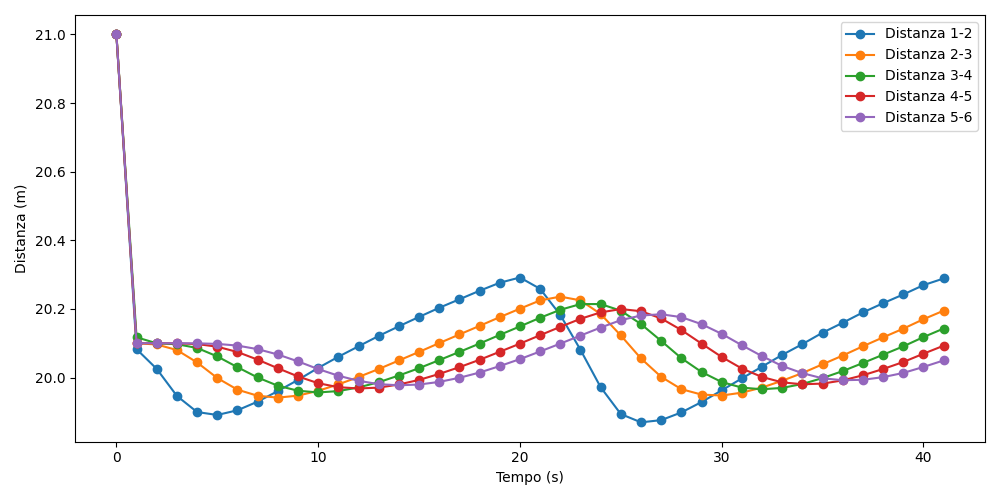
\includegraphics[width=0.96\textwidth]{images/5-experiment/car-spacing/distance_20.png}
    \caption{Distanze con $20.0 m$ come distanza iniziale.}
    \label{fig:20-space-distance}
\end{figure}

\begin{figure}[H]
    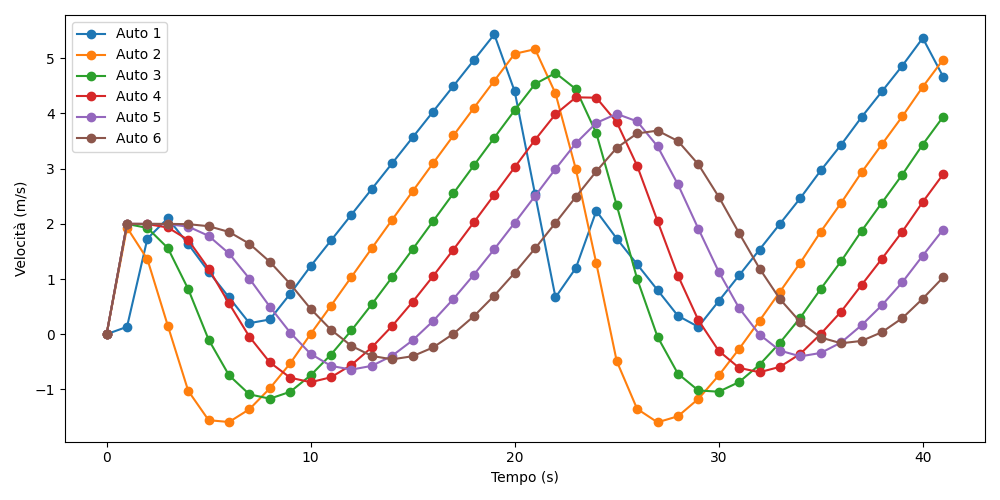
\includegraphics[width=0.96\textwidth]{images/5-experiment/car-spacing/velocity_20.png}
    \caption{Velocità con distanza iniziale $20.0 m$.}
    \label{fig:20-space-velocity}
\end{figure}
\vspace*{\fill}
\newpage

% DELAY %

\subsubsection{Ritardo di comunicazione}
\vspace*{\fill}
\begin{table}[h]
    \centering
    \begin{tabular}{|c|c|c|c|}
        \hline
        N° auto & Distanza Iniziale & Distanza Target & Ritardo \\
        \hline
        $6$ & $6.0 m$ & $5.0 m$ & $0.5 s$ \\
        \hline
        $Time\hspace{0.2em}Headway$ & $\tau$ & $K_p$ & $K_d$  \\
        \hline
        $0.5$ & $0.1$ & $0.2$ & $0.7$ \\
        \hline
    \end{tabular}
\end{table}

\begin{figure}[H]
    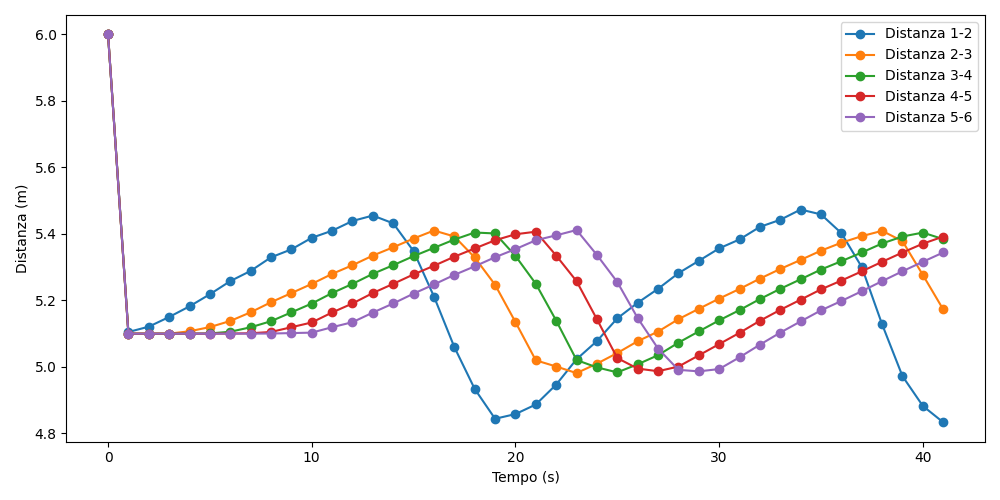
\includegraphics[width=0.96\textwidth]{images/5-experiment/delay/distance_0,5.png}
    \caption{Distanze con ritardo a $0.5 s$.}
    \label{fig:0.5-delay-distance}
\end{figure}

\begin{figure}[H]
    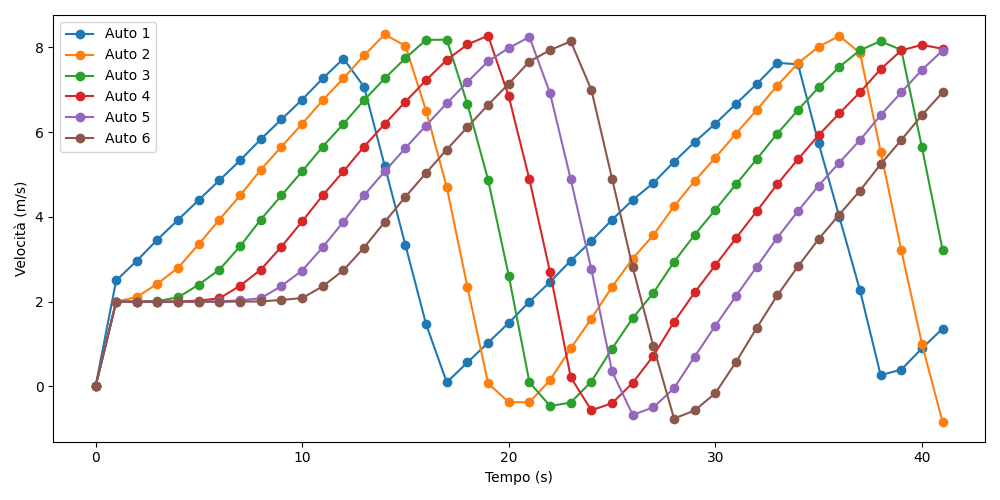
\includegraphics[width=0.96\textwidth]{images/5-experiment/delay/velocity_0,5.png}
    \caption{Velocità con ritardo a $0.5 s$.}
    \label{fig:0.5-delay-velocity}
\end{figure}
\vspace*{\fill}
\newpage
\vspace*{\fill}
\begin{table}[h]
    \centering
    \begin{tabular}{|c|c|c|c|}
        \hline
        N° auto & Distanza Iniziale & Distanza Target & Ritardo \\
        \hline
        $6$ & $6.0 m$ & $5.0 m$ & $1 s$ \\
        \hline
        $Time\hspace{0.2em}Headway$ & $\tau$ & $K_p$ & $K_d$  \\
        \hline
        $0.5$ & $0.1$ & $0.2$ & $0.7$ \\
        \hline
    \end{tabular}
\end{table}

\begin{figure}[H]
    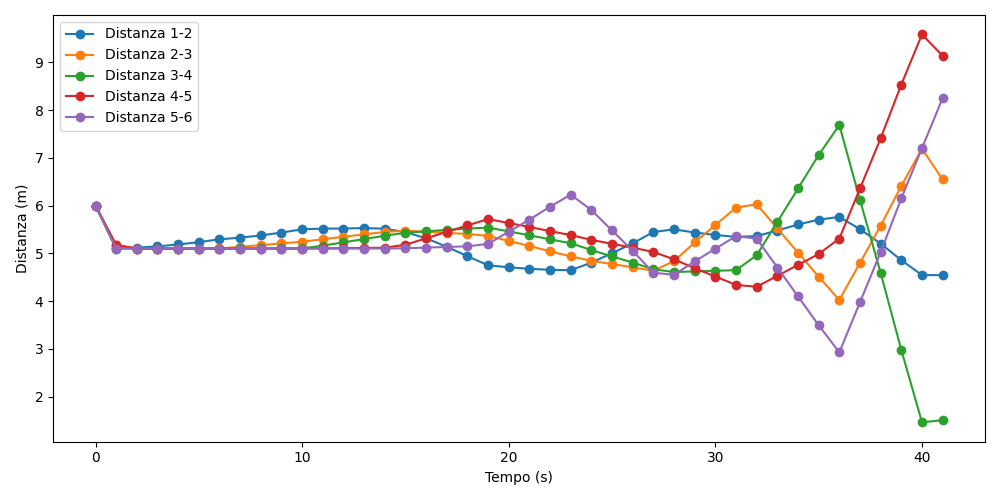
\includegraphics[width=0.96\textwidth]{images/5-experiment/delay/distance_1.png}
    \caption{Distanze con ritardo a $1 s$.}
    \label{fig:1-delay-distance}
\end{figure}

\begin{figure}[H]
    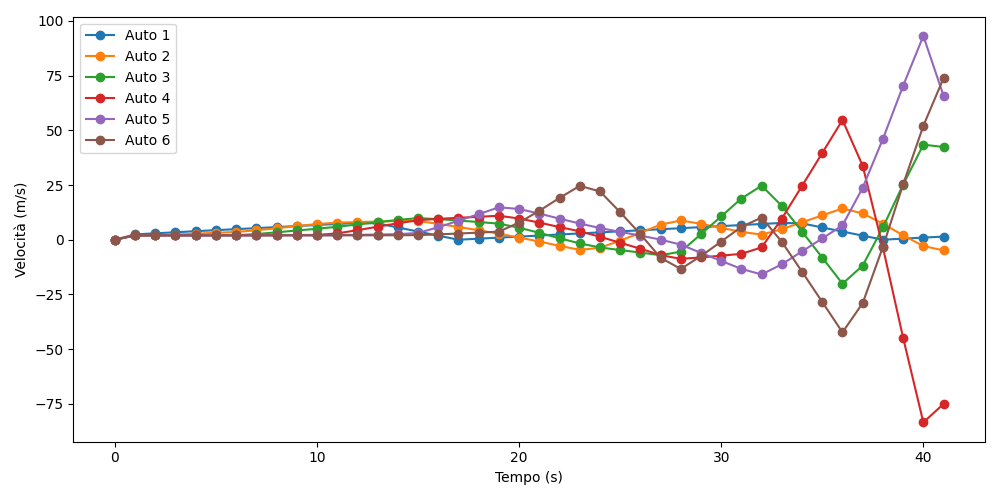
\includegraphics[width=0.96\textwidth]{images/5-experiment/delay/velocity_1.png}
    \caption{Velocità con ritardo a $1 s$.}
    \label{fig:1-delay-velocity}
\end{figure}
\vspace*{\fill}
\newpage

% TIME HEADWAY %

\subsubsection{Time Headway}
\vspace*{\fill}
\begin{table}[h]
    \centering
    \begin{tabular}{|c|c|c|c|}
        \hline
        N° auto & Distanza Iniziale & Distanza Target & Ritardo \\
        \hline
        $6$ & $6.0 m$ & $5.0 m$ & $0.2 s$ \\
        \hline
        $Time\hspace{0.2em}Headway$ & $\tau$ & $K_p$ & $K_d$  \\
        \hline
        $0.05$ & $0.1$ & $0.2$ & $0.7$ \\
        \hline
    \end{tabular}
\end{table}

\begin{figure}[H]
    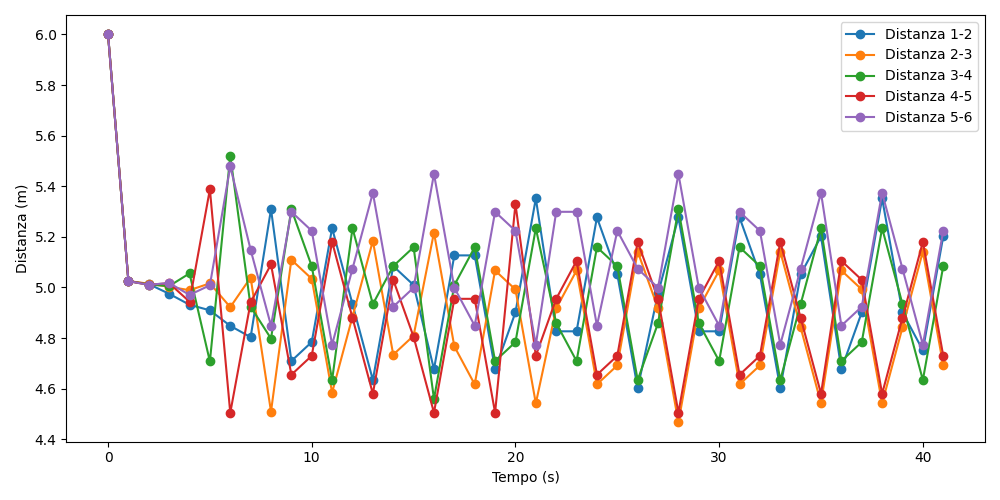
\includegraphics[width=0.96\textwidth]{images/5-experiment/time-headway/distance_0,05.png}
    \caption{Distanze con $Time\hspace{0.2em}Headway$ a $0.05$.}
    \label{fig:0.05-headway-distance}
\end{figure}

\begin{figure}[H]
    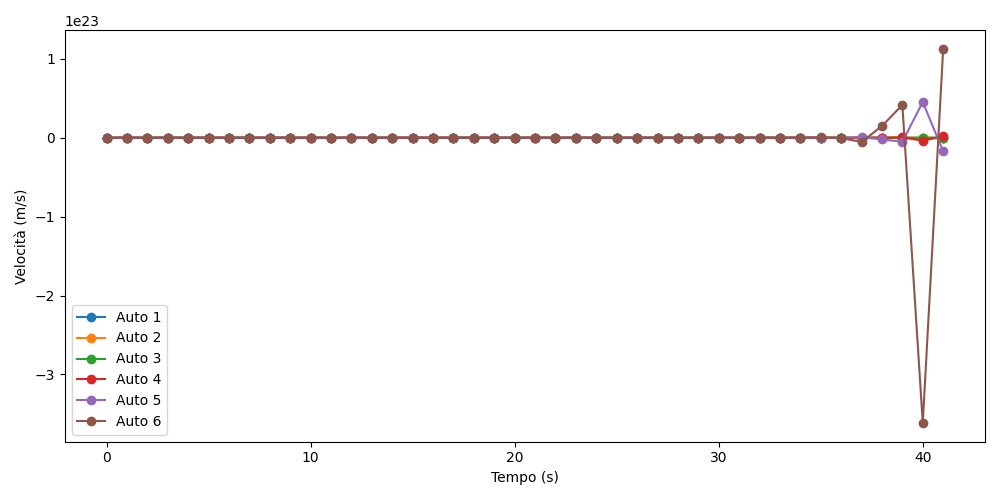
\includegraphics[width=0.96\textwidth]{images/5-experiment/time-headway/velocity_0,05.png}
    \caption{Velocità con $Time\hspace{0.2em}Headway$ a $0.05$.}
    \label{fig:0.05-headway-velocity}
\end{figure}
\vspace*{\fill}
\newpage
\vspace*{\fill}
\begin{table}[h]
    \centering
    \begin{tabular}{|c|c|c|c|}
        \hline
        N° auto & Distanza Iniziale & Distanza Target & Ritardo \\
        \hline
        $6$ & $6.0 m$ & $5.0 m$ & $0.2 s$ \\
        \hline
        $Time\hspace{0.2em}Headway$ & $\tau$ & $K_p$ & $K_d$  \\
        \hline
        $0.1$ & $0.1$ & $0.2$ & $0.7$ \\
        \hline
    \end{tabular}
\end{table}

\begin{figure}[H]
    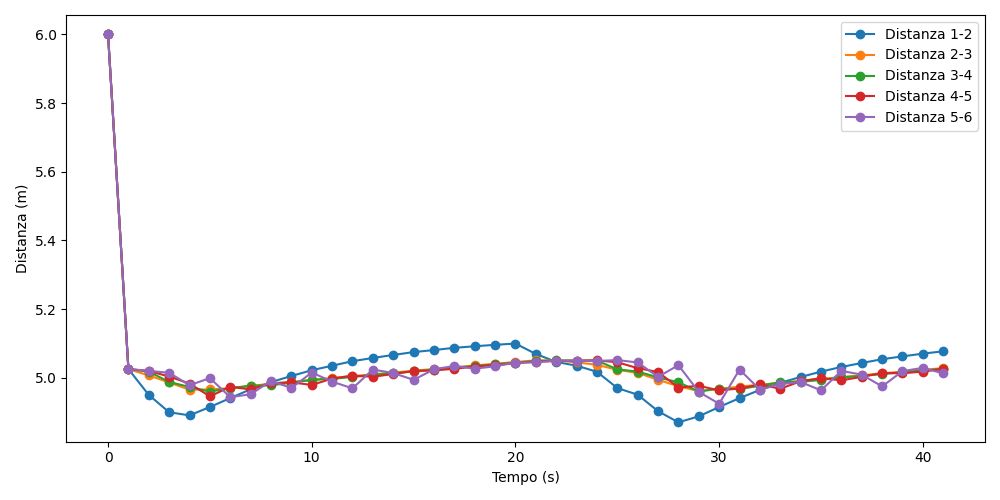
\includegraphics[width=0.96\textwidth]{images/5-experiment/time-headway/distance_0,1.png}
    \caption{Distanze con $Time\hspace{0.2em}Headway$ a $0.1$.}
    \label{fig:0.1-headway-distance}
\end{figure}

\begin{figure}[H]
    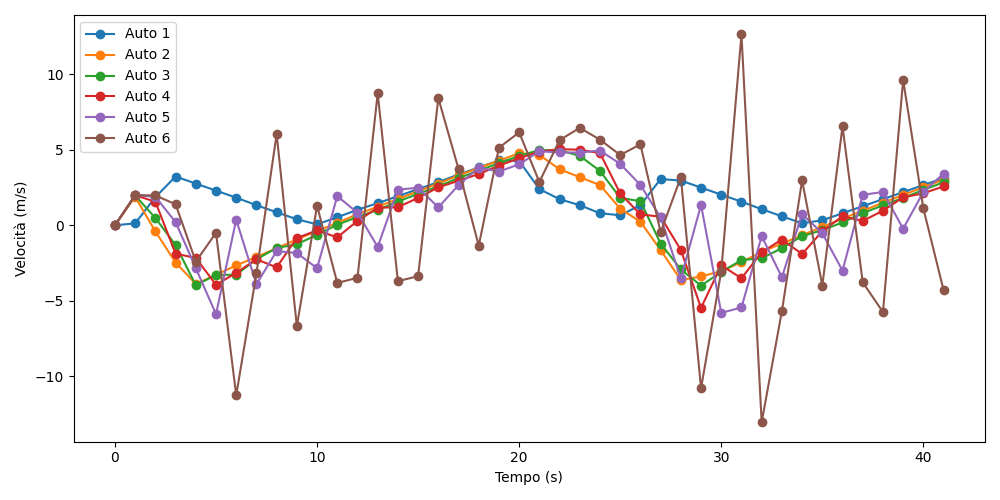
\includegraphics[width=0.96\textwidth]{images/5-experiment/time-headway/velocity_0,1.png}
    \caption{Velocità con $Time\hspace{0.2em}Headway$ a $0.1$.}
    \label{fig:0.1-headway-velocity}
\end{figure}
\vspace*{\fill}
\newpage
\vspace*{\fill}
\begin{table}[h]
    \centering
    \begin{tabular}{|c|c|c|c|}
        \hline
        N° auto & Distanza Iniziale & Distanza Target & Ritardo \\
        \hline
        $6$ & $6.0 m$ & $5.0 m$ & $0.2 s$ \\
        \hline
        $Time\hspace{0.2em}Headway$ & $\tau$ & $K_p$ & $K_d$  \\
        \hline
        $1$ & $0.1$ & $0.2$ & $0.7$ \\
        \hline
    \end{tabular}
\end{table}

\begin{figure}[H]
    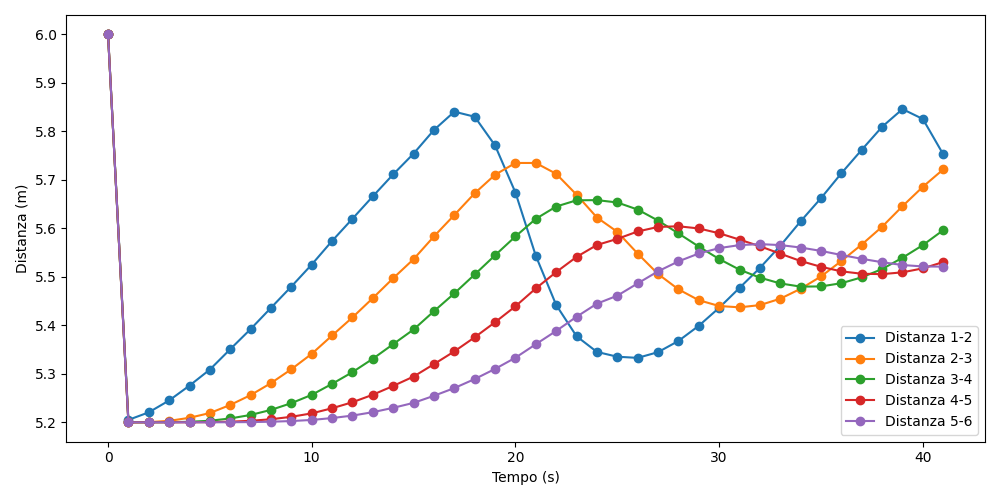
\includegraphics[width=0.96\textwidth]{images/5-experiment/time-headway/distance_1.png}
    \caption{Distanze con $Time\hspace{0.2em}Headway$ a $1$.}
    \label{fig:1-headway-distance}
\end{figure}

\begin{figure}[H]
    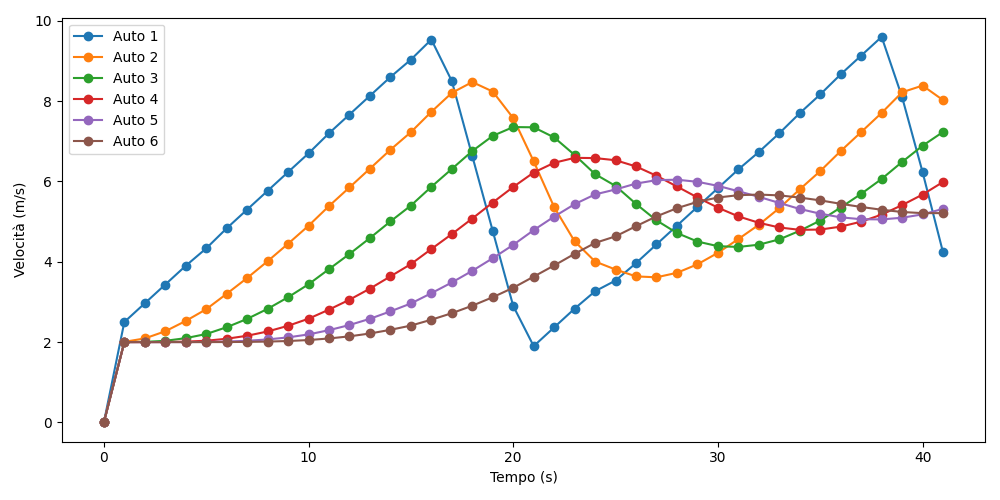
\includegraphics[width=0.96\textwidth]{images/5-experiment/time-headway/velocity_1.png}
    \caption{Velocità con $Time\hspace{0.2em}Headway$ a $1$.}
    \label{fig:1-headway-velocity}
\end{figure}
\vspace*{\fill}
\newpage
\vspace*{\fill}
\begin{table}[h]
    \centering
    \begin{tabular}{|c|c|c|c|}
        \hline
        N° auto & Distanza Iniziale & Distanza Target & Ritardo \\
        \hline
        $6$ & $6.0 m$ & $5.0 m$ & $0.2 s$ \\
        \hline
        $Time\hspace{0.2em}Headway$ & $\tau$ & $K_p$ & $K_d$  \\
        \hline
        $2$ & $0.1$ & $0.2$ & $0.7$ \\
        \hline
    \end{tabular}
\end{table}

\begin{figure}[H]
    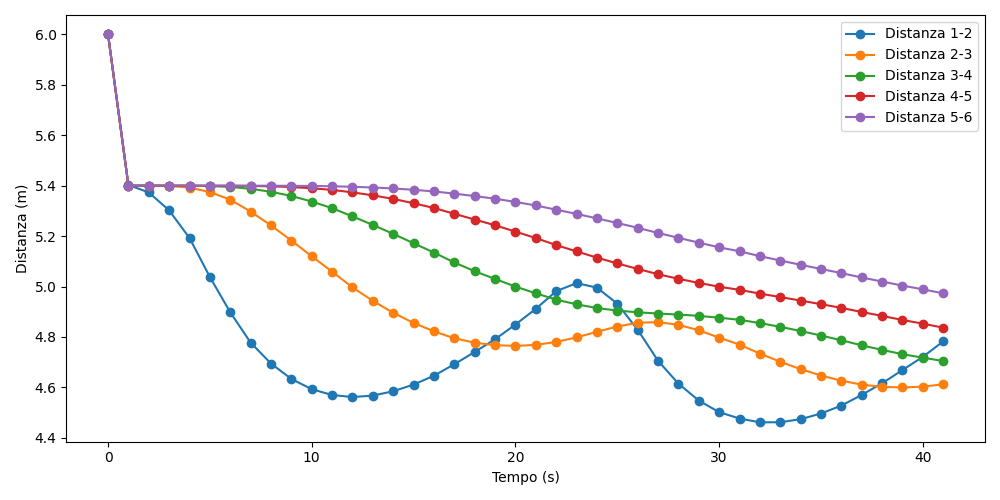
\includegraphics[width=0.96\textwidth]{images/5-experiment/time-headway/distance_2.png}
    \caption{Distanze con $Time\hspace{0.2em}Headway$ a $2$.}
    \label{fig:2-headway-distance}
\end{figure}

\begin{figure}[H]
    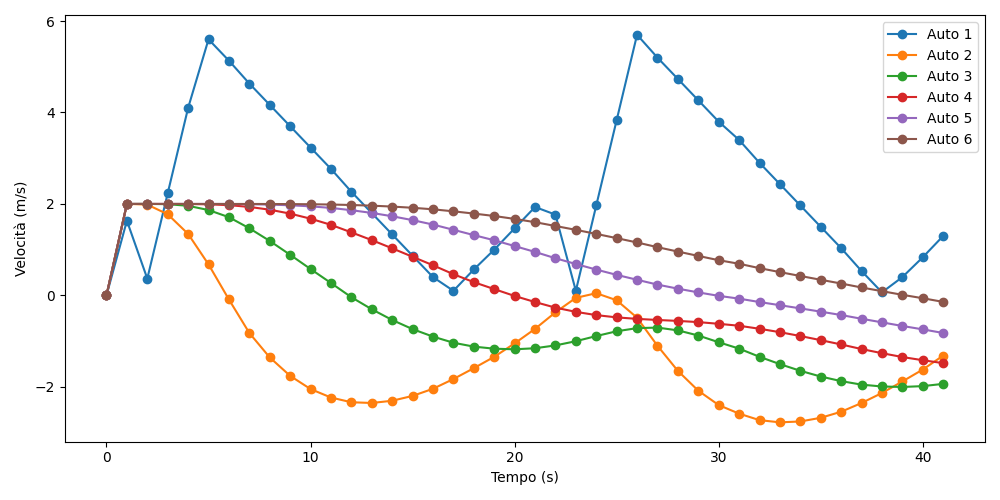
\includegraphics[width=0.96\textwidth]{images/5-experiment/time-headway/velocity_2.png}
    \caption{Velocità con $Time\hspace{0.2em}Headway$ a $2$.}
    \label{fig:2-headway-velocity}
\end{figure}
\vspace*{\fill}
\newpage

% TAU %

\subsubsection{Tau \texorpdfstring{($\tau$)}{}}
\vspace*{\fill}
\begin{table}[h]
    \centering
    \begin{tabular}{|c|c|c|c|}
        \hline
        N° auto & Distanza Iniziale & Distanza Target & Ritardo \\
        \hline
        $6$ & $6.0 m$ & $5.0 m$ & $0.2 s$ \\
        \hline
        $Time\hspace{0.2em}Headway$ & $\tau$ & $K_p$ & $K_d$  \\
        \hline
        $0.5$ & $0.01$ & $0.2$ & $0.7$ \\
        \hline
    \end{tabular}
\end{table}

\begin{figure}[H]
    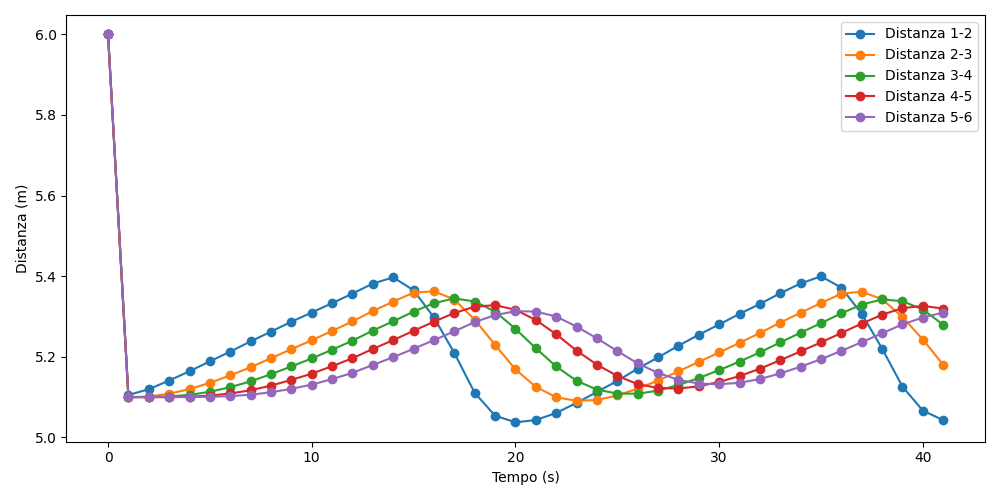
\includegraphics[width=0.96\textwidth]{images/5-experiment/tau/distance_0,01.png}
    \caption{Distanze con $\tau$ a $0.01$.}
    \label{fig:0.01-tau-distance}
\end{figure}

\begin{figure}[H]
    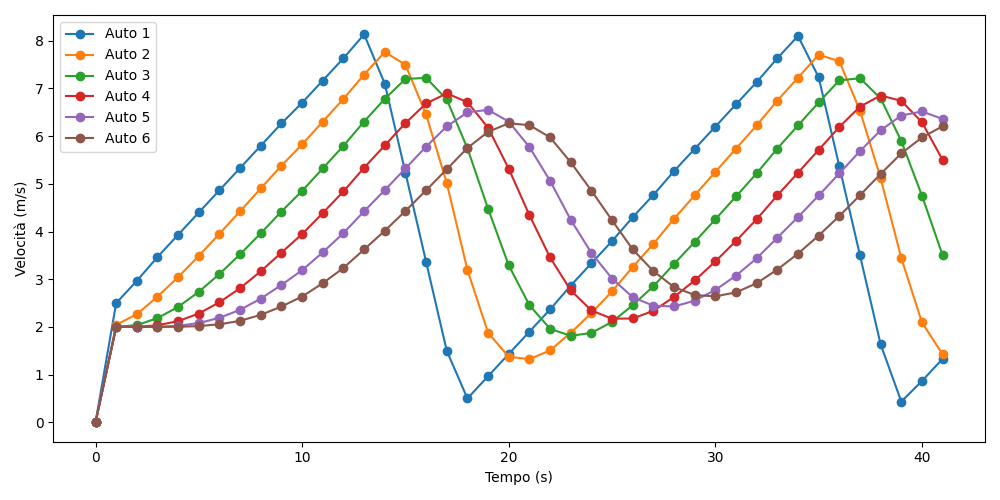
\includegraphics[width=0.96\textwidth]{images/5-experiment/tau/velocity_0,01.png}
    \caption{Velocità con $\tau$ a $0.01$.}
    \label{fig:0.01-tau-velocity}
\end{figure}
\vspace*{\fill}
\newpage
\vspace*{\fill}
\begin{table}[h]
    \centering
    \begin{tabular}{|c|c|c|c|}
        \hline
        N° auto & Distanza Iniziale & Distanza Target & Ritardo \\
        \hline
        $6$ & $6.0 m$ & $5.0 m$ & $0.2 s$ \\
        \hline
        $Time\hspace{0.2em}Headway$ & $\tau$ & $K_p$ & $K_d$  \\
        \hline
        $0.5$ & $0.7$ & $0.2$ & $0.7$ \\
        \hline
    \end{tabular}
\end{table}
\begin{figure}[H]
    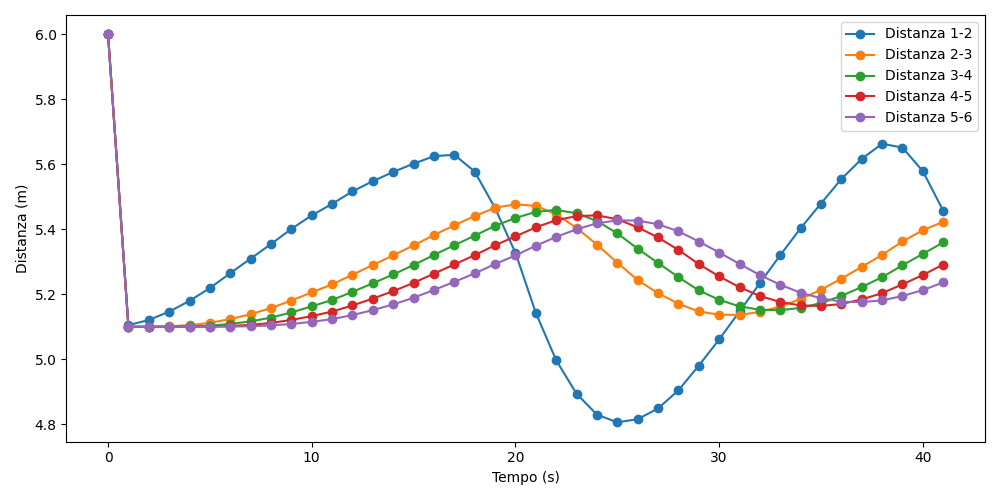
\includegraphics[width=0.96\textwidth]{images/5-experiment/tau/distance_0,7.png}
    \caption{Distanze con $\tau$ a $0.7$.}
    \label{fig:0.7-tau-distance}
\end{figure}

\begin{figure}[H]
    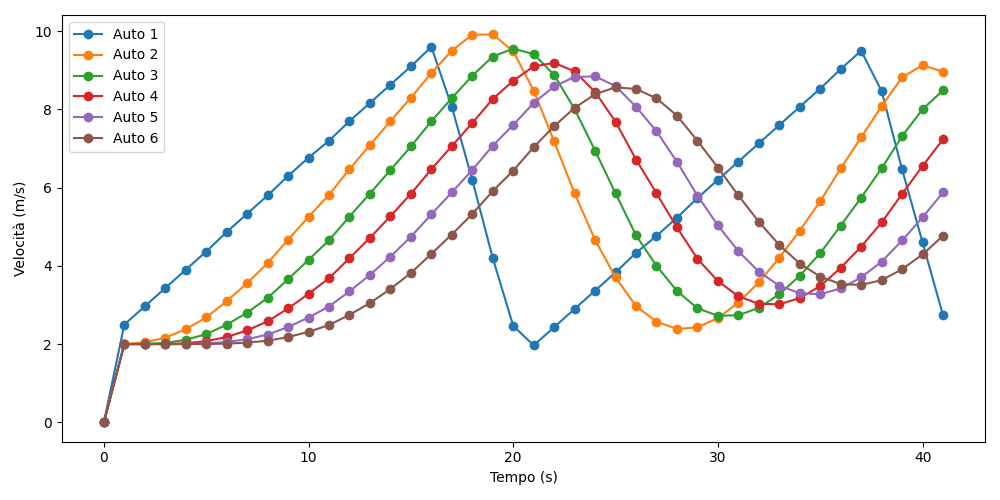
\includegraphics[width=0.96\textwidth]{images/5-experiment/tau/velocity_0,7.png}
    \caption{Velocità con $\tau$ a $0.7$.}
    \label{fig:0.7-tau-velocity}
\end{figure}
\vspace*{\fill}
\newpage
\vspace*{\fill}
\begin{table}[h]
    \centering
    \begin{tabular}{|c|c|c|c|}
        \hline
        N° auto & Distanza Iniziale & Distanza Target & Ritardo \\
        \hline
        $6$ & $6.0 m$ & $5.0 m$ & $0.2 s$ \\
        \hline
        $Time\hspace{0.2em}Headway$ & $\tau$ & $K_p$ & $K_d$  \\
        \hline
        $0.5$ & $2.0$ & $0.2$ & $0.7$ \\
        \hline
    \end{tabular}
\end{table}

\begin{figure}[H]
    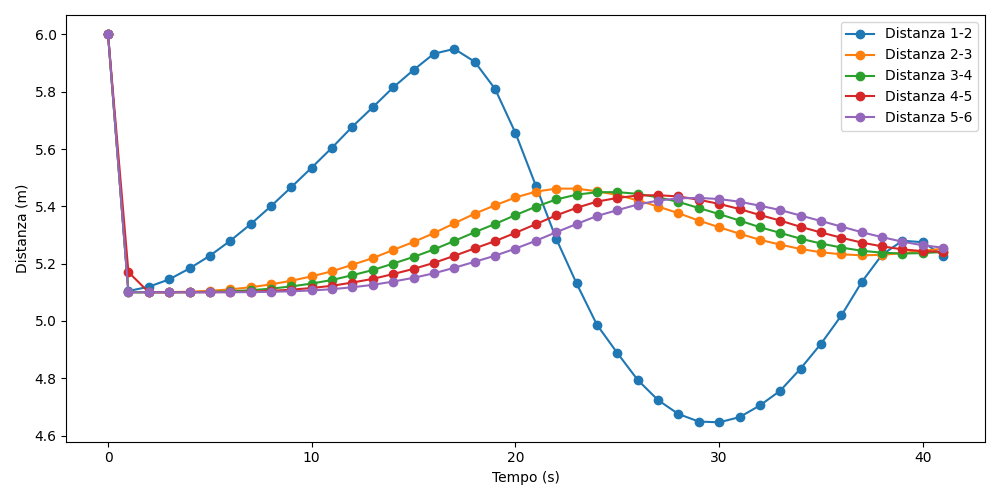
\includegraphics[width=0.96\textwidth]{images/5-experiment/tau/distance_2.png}
    \caption{Distanze con $\tau$ a $2.0$.}
    \label{fig:2-tau-distance}
\end{figure}

\begin{figure}[H]
    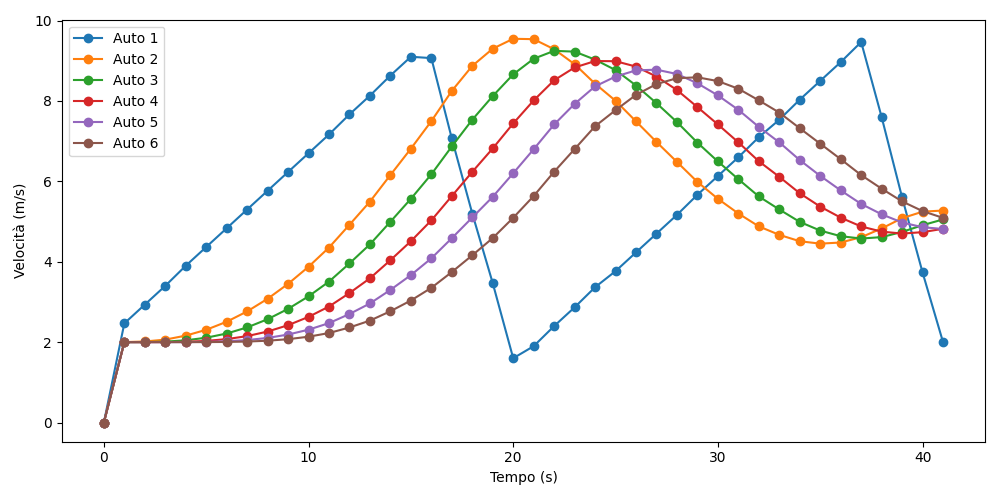
\includegraphics[width=0.96\textwidth]{images/5-experiment/tau/velocity_2.png}
    \caption{Velocità con $\tau$ a $2.0$.}
    \label{fig:2-tau-velocity}
\end{figure}
\vspace*{\fill}
\newpage


% VELOCITÀ CON PARAMETRI DEFAULT %

\subsubsection{Velocità con parametri di default}

\begin{table}[h]
    \centering
    \begin{tabular}{|c|c|c|c|c|}
        \hline
        Velocità $t1$ & Velocità $t2$ & Velocità $t3$ &Velocità $t4$ &Velocità $t5$\\
        \hline
            $0\hspace{0.2em}m/s$ & $0\hspace{0.2em}m/s$ & $0\hspace{0.2em}m/s$ & $0\hspace{0.2em}m/s$ & $0\hspace{0.2em}m/s$ \\
        \hline
    \end{tabular}
\end{table}
\begin{table}[h]
    \centering
    \begin{tabular}{|c|c|c|c|}
        \hline
        N° auto & Distanza Iniziale & Distanza Target & Ritardo \\
        \hline
        $6$ & $6.0 m$ & $5.0 m$ & $0.2 s$ \\
        \hline
        $Time\hspace{0.2em}Headway$ & $\tau$ & $K_p$ & $K_d$  \\
        \hline
        $0.5$ & $0.1$ & $0.2$ & $0.7$ \\
        \hline
    \end{tabular}
\end{table}

\begin{figure}[H]
    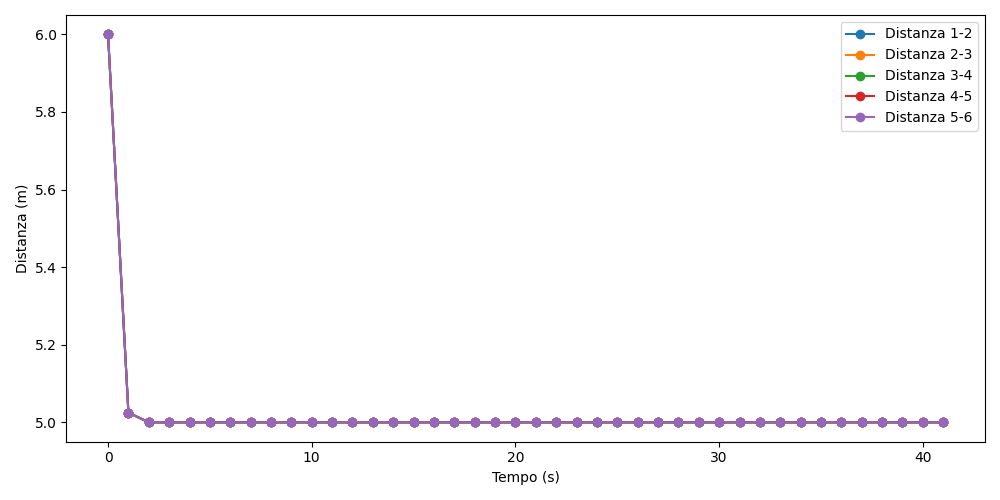
\includegraphics[width=0.96\textwidth]{images/5-experiment/velocity/distance_0-0-0-0-0.png}
    \caption{Distanze con primo veicolo fermo.}
    \label{fig:0-constvelocity-distance}
\end{figure}

\begin{figure}[H]
    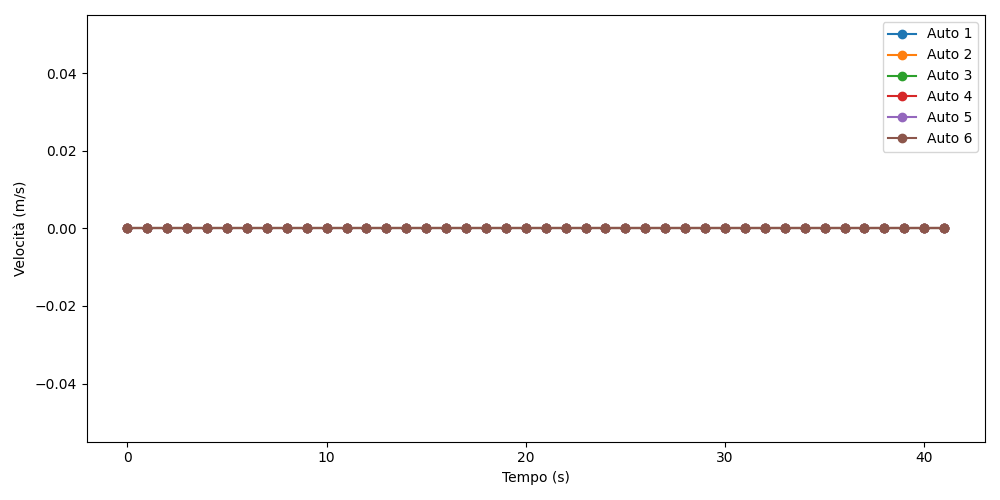
\includegraphics[width=0.96\textwidth]{images/5-experiment/velocity/velocity_0-0-0-0-0.png}
    \caption{Velocità con primo veicolo fermo.}
    \label{fig:0-constvelocity-velocity}
\end{figure}

\newpage

\begin{table}[h]
    \centering
    \begin{tabular}{|c|c|c|c|c|}
        \hline
        Velocità $t1$ & Velocità $t2$ & Velocità $t3$ &Velocità $t4$ &Velocità $t5$\\
        \hline
            $10\hspace{0.2em}m/s$ & $10\hspace{0.2em}m/s$ & $10\hspace{0.2em}m/s$ & $10\hspace{0.2em}m/s$ & $10\hspace{0.2em}m/s$ \\
        \hline
    \end{tabular}
\end{table}
\begin{table}[h]
    \centering
    \begin{tabular}{|c|c|c|c|}
        \hline
        N° auto & Distanza Iniziale & Distanza Target & Ritardo \\
        \hline
        $6$ & $6.0 m$ & $5.0 m$ & $0.2 s$ \\
        \hline
        $Time\hspace{0.2em}Headway$ & $\tau$ & $K_p$ & $K_d$  \\
        \hline
        $0.5$ & $0.1$ & $0.2$ & $0.7$ \\
        \hline
    \end{tabular}
\end{table}

\begin{figure}[H]
    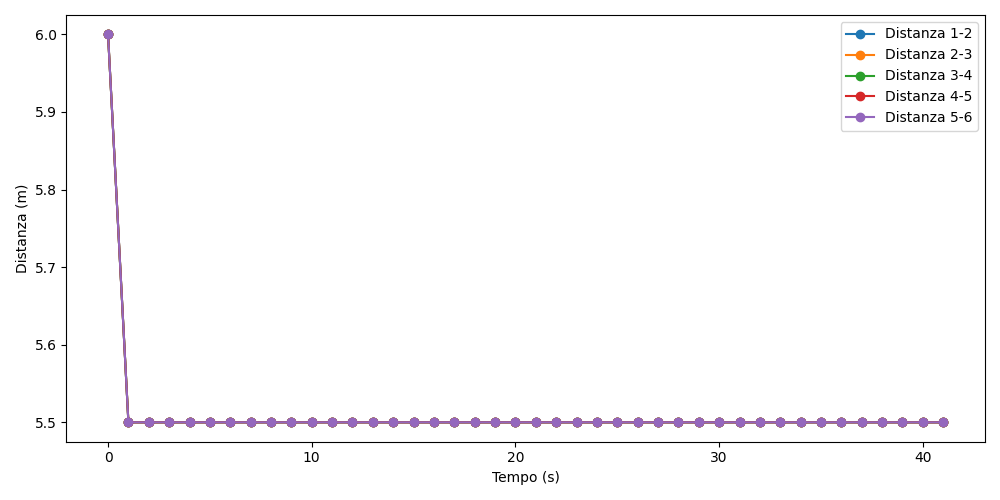
\includegraphics[width=0.96\textwidth]{images/5-experiment/velocity/distance_10-10-10-10-10.png}
    \caption{Distanze con velocità costante a $10\hspace{0.2em}m/s$.}
    \label{fig:10-constvelocity-distance}
\end{figure}

\begin{figure}[H]
    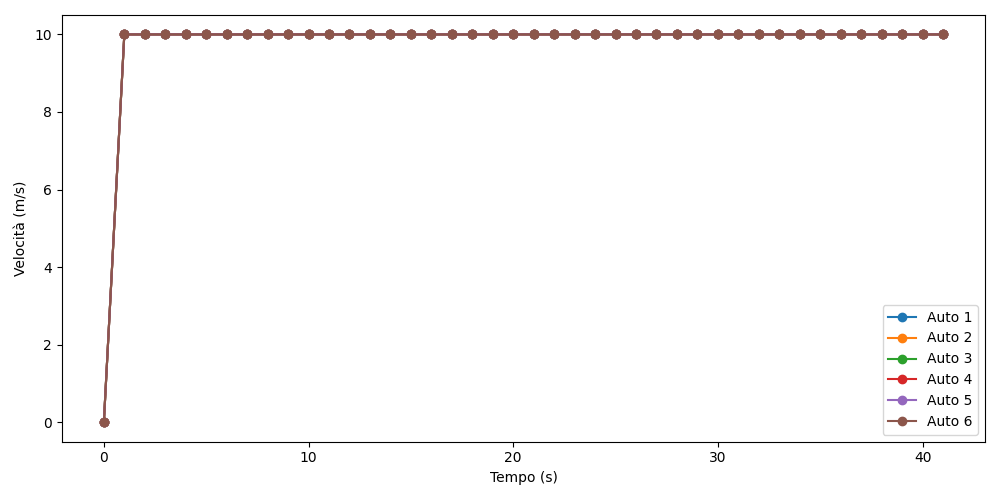
\includegraphics[width=0.96\textwidth]{images/5-experiment/velocity/velocity_10-10-10-10-10.png}
    \caption{Velocità con velocità costante a $10\hspace{0.2em}m/s$.}
    \label{fig:10-constvelocity-velocity}
\end{figure}

\newpage

\begin{table}[h]
    \centering
    \begin{tabular}{|c|c|c|c|c|}
        \hline
        Velocità $t1$ & Velocità $t2$ & Velocità $t3$ &Velocità $t4$ &Velocità $t5$\\
        \hline
            $35\hspace{0.2em}m/s$ & $35\hspace{0.2em}m/s$ & $35\hspace{0.2em}m/s$ & $35\hspace{0.2em}m/s$ & $35\hspace{0.2em}m/s$ \\
        \hline
    \end{tabular}
\end{table}
\begin{table}[h]
    \centering
    \begin{tabular}{|c|c|c|c|}
        \hline
        N° auto & Distanza Iniziale & Distanza Target & Ritardo \\
        \hline
        $6$ & $6.0 m$ & $5.0 m$ & $0.2 s$ \\
        \hline
        $Time\hspace{0.2em}Headway$ & $\tau$ & $K_p$ & $K_d$  \\
        \hline
        $0.5$ & $0.1$ & $0.2$ & $0.7$ \\
        \hline
    \end{tabular}
\end{table}

\begin{figure}[H]
    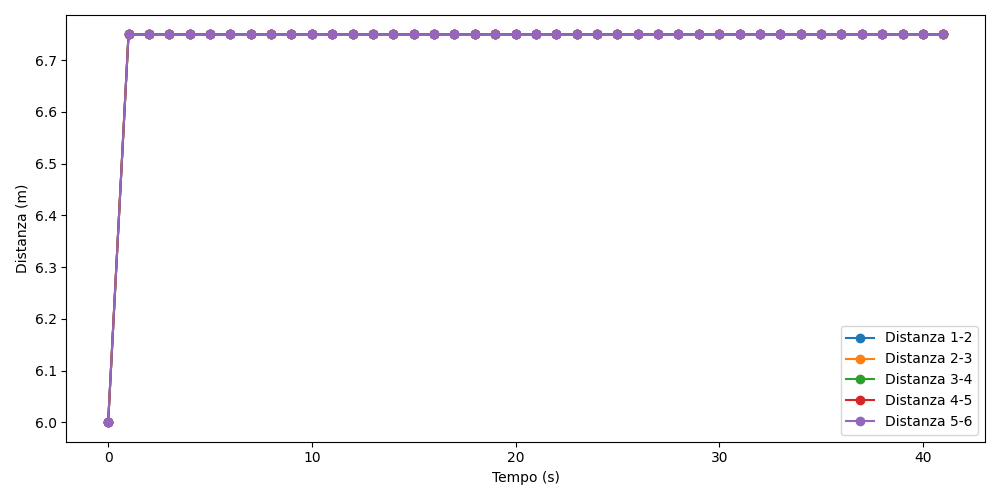
\includegraphics[width=0.96\textwidth]{images/5-experiment/velocity/distance_35-35-35-35-35.png}
    \caption{Distanze con velocità costante a $35\hspace{0.2em}m/s$.}
    \label{fig:35-constvelocity-distance}
\end{figure}

\begin{figure}[H]
    \includegraphics[width=0.96\textwidth]{images/5-experiment/velocity/velocity_35-35-35-35-35.png}
    \caption{Velocità con velocità costante a $35\hspace{0.2em}m/s$.}
    \label{fig:35-constvelocity-velocity}
\end{figure}

\newpage

\begin{table}[h]
    \centering
    \begin{tabular}{|c|c|c|c|c|}
        \hline
        Velocità $t1$ & Velocità $t2$ & Velocità $t3$ &Velocità $t4$ &Velocità $t5$\\
        \hline
            $20\hspace{0.2em}m/s$ & $0\hspace{0.2em}m/s$ & $20\hspace{0.2em}m/s$ & $0\hspace{0.2em}m/s$ & $20\hspace{0.2em}m/s$ \\
        \hline
    \end{tabular}
\end{table}
\begin{table}[h]
    \centering
    \begin{tabular}{|c|c|c|c|}
        \hline
        N° auto & Distanza Iniziale & Distanza Target & Ritardo \\
        \hline
        $6$ & $6.0 m$ & $5.0 m$ & $0.2 s$ \\
        \hline
        $Time\hspace{0.2em}Headway$ & $\tau$ & $K_p$ & $K_d$ \\
        \hline
        $0.5$ & $0.1$ & $0.2$ & $0.7$ \\
        \hline
    \end{tabular}
\end{table}

\begin{figure}[H]
    \includegraphics[width=0.96\textwidth]{images/5-experiment/velocity/distance_20-0-20-0-20.png}
    \caption{Distanze con velocità variabile tra $20\hspace{0.2em}m/s$ e $0\hspace{0.2em}m/s$.}
    \label{fig:20-0-variabvelocity-distance}
\end{figure}

\begin{figure}[H]
    \includegraphics[width=0.96\textwidth]{images/5-experiment/velocity/velocity_20-0-20-0-20.png}
    \caption{Velocità con velocità variabile tra $20\hspace{0.2em}m/s$ e $0\hspace{0.2em}m/s$.}
    \label{fig:20-0-variabvelocity-velocity}
\end{figure}

\newpage

\begin{table}[h]
    \centering
    \begin{tabular}{|c|c|c|c|c|}
        \hline
        Velocità $t1$ & Velocità $t2$ & Velocità $t3$ &Velocità $t4$ &Velocità $t5$\\
        \hline
            $35\hspace{0.2em}m/s$ & $35\hspace{0.2em}m/s$ & $0\hspace{0.2em}m/s$ & $35\hspace{0.2em}m/s$ & $35\hspace{0.2em}m/s$ \\
        \hline
    \end{tabular}
\end{table}
\begin{table}[h]
    \centering
    \begin{tabular}{|c|c|c|c|}
        \hline
        N° auto & Distanza Iniziale & Distanza Target & Ritardo \\
        \hline
        $6$ & $6.0 m$ & $5.0 m$ & $0.2 s$ \\
        \hline
        $Time\hspace{0.2em}Headway$ & $\tau$ & $K_p$ & $K_d$  \\
        \hline
        $0.5$ & $0.1$ & $0.2$ & $0.7$ \\
        \hline
    \end{tabular}
\end{table}

\begin{figure}[H]
    \includegraphics[width=0.96\textwidth]{images/5-experiment/velocity/distance_35-35-0-35-35.png}
    \caption{Distanze con velocità variabile tra $35\hspace{0.2em}m/s$ e $0\hspace{0.2em}m/s$.}
    \label{fig:35-35-0-variabvelocity-distance}
\end{figure}

\begin{figure}[H]
    \includegraphics[width=0.96\textwidth]{images/5-experiment/velocity/velocity_35-35-0-35-35.png}
    \caption{Velocità con velocità variabile tra $35\hspace{0.2em}m/s$ e $0\hspace{0.2em}m/s$.}
    \label{fig:35-35-0-variabvelocity-velocity}
\end{figure}

\newpage


% VELOCITÀ NON PARAMETRI DEFAULT%

\subsubsection{Velocità con parametri diversi da quelli di default}

\begin{table}[h]
    \centering
    \begin{tabular}{|c|c|c|c|c|}
        \hline
        Velocità $t1$ & Velocità $t2$ & Velocità $t3$ &Velocità $t4$ &Velocità $t5$\\
        \hline
            $15\hspace{0.2em}m/s$ & $15\hspace{0.2em}m/s$ & $15\hspace{0.2em}m/s$ & $15\hspace{0.2em}m/s$ & $15\hspace{0.2em}m/s$ \\
        \hline
    \end{tabular}
\end{table}
\begin{table}[h]
    \centering
    \begin{tabular}{|c|c|c|c|}
        \hline
        N° auto & Distanza Iniziale & Distanza Target & Ritardo \\
        \hline
        $10$ & $6.0 m$ & $5.0 m$ & $0.2 s$ \\
        \hline
        $Time\hspace{0.2em}Headway$ & $\tau$ & $K_p$ & $K_d$  \\
        \hline
        $0.1$ & $0.1$ & $0.2$ & $0.7$ \\
        \hline
    \end{tabular}
\end{table}

\begin{figure}[H]
    \includegraphics[width=0.96\textwidth]{images/5-experiment/compost/distance_a.png}
    \caption{Distanze con velocità costante a $15\hspace{0.2em}m/s$.}
    \label{fig:a-compost-distance}
\end{figure}

\begin{figure}[H]
    \includegraphics[width=0.96\textwidth]{images/5-experiment/compost/velocity_a.png}
    \caption{Velocità con velocità costante a $15\hspace{0.2em}m/s$.}
    \label{fig:a-compost-velocity}
\end{figure}

\vspace*{\fill}
\newpage
\vspace*{\fill}
\begin{table}[h]
    \centering
    \begin{tabular}{|c|c|c|c|c|}
        \hline
        Velocità $t1$ & Velocità $t2$ & Velocità $t3$ &Velocità $t4$ &Velocità $t5$\\
        \hline
            $25\hspace{0.2em}m/s$ & $25\hspace{0.2em}m/s$ & $25\hspace{0.2em}m/s$ & $25\hspace{0.2em}m/s$ & $25\hspace{0.2em}m/s$ \\
        \hline
    \end{tabular}
\end{table}
\begin{table}[h]
    \centering
    \begin{tabular}{|c|c|c|c|}
        \hline
        N° auto & Distanza Iniziale & Distanza Target & Ritardo \\
        \hline
        $10$ & $3.0 m$ & $2.0 m$ & $0.2 s$ \\
        \hline
        $Time\hspace{0.2em}Headway$ & $\tau$ & $K_p$ & $K_d$  \\
        \hline
        $0.1$ & $0.1$ & $0.2$ & $0.7$ \\
        \hline
    \end{tabular}
\end{table}

\begin{figure}[H]
    \includegraphics[width=0.96\textwidth]{images/5-experiment/compost/distance_b.png}
    \caption{Distanze con velocità costante a $25\hspace{0.2em}m/s$.}
    \label{fig:b-compost-distance}
\end{figure}

\begin{figure}[H]
    \includegraphics[width=0.96\textwidth]{images/5-experiment/compost/velocity_b.png}
    \caption{Velocità con velocità costante a $25\hspace{0.2em}m/s$.}
    \label{fig:b-compost-velocity}
\end{figure}
\vspace*{\fill}
\newpage

\begin{table}[h]
    \centering
    \begin{tabular}{|c|c|c|c|c|}
        \hline
        Velocità $t1$ & Velocità $t2$ & Velocità $t3$ &Velocità $t4$ &Velocità $t5$\\
        \hline
            $25\hspace{0.2em}m/s$ & $25\hspace{0.2em}m/s$ & $15\hspace{0.2em}m/s$ & $25\hspace{0.2em}m/s$ & $25\hspace{0.2em}m/s$ \\
        \hline
    \end{tabular}
\end{table}

\begin{table}[h]
    \centering
    \begin{tabular}{|c|c|c|c|}
        \hline
        N° auto & Distanza Iniziale & Distanza Target & Ritardo \\
        \hline
        $10$ & $3.0 m$ & $5.0 m$ & $0.2 s$ \\
        \hline
        $Time\hspace{0.2em}Headway$ & $\tau$ & $K_p$ & $K_d$  \\
        \hline
        $0.1$ & $0.1$ & $0.2$ & $0.7$ \\
        \hline
    \end{tabular}
\end{table}

\begin{figure}[H]
    \includegraphics[width=0.96\textwidth]{images/5-experiment/compost/distance_c.png}
    \caption{Distanze con velocità variabile tra $15\hspace{0.2em}m/s$ e $25\hspace{0.2em}m/s$.}
    \label{fig:c-compost-distance}
\end{figure}

\begin{figure}[H]
    \includegraphics[width=0.96\textwidth]{images/5-experiment/compost/velocity_c.png}
    \caption{Velocità con velocità variabile tra $15\hspace{0.2em}m/s$ e $25\hspace{0.2em}m/s$.}
    \label{fig:c-compost-velocity}
\end{figure}

\newpage


% MODELLO INSTABILE %

\subsection{Modello instabile}

% DELAY %

\subsubsection{Ritardo di comunicazione}
\vspace*{\fill}
\begin{table}[h]
    \centering
    \begin{tabular}{|c|c|c|c|}
        \hline
        N° auto & Distanza Iniziale & Distanza Target & Ritardo \\
        \hline
        $6$ & $6.0 m$ & $5.0 m$ & $1.5 s$ \\
        \hline
        $Time\hspace{0.2em}Headway$ & $\tau$ & $K_p$ & $K_d$  \\
        \hline
        $0.5$ & $0.1$ & $0.2$ & $0.7$ \\
        \hline
    \end{tabular}
\end{table}

\begin{figure}[H]
    \includegraphics[width=0.96\textwidth]{images/5-experiment/delay/distance_1,5+.png}
    \caption{Distanze con ritardo a $1.5 s$.}
    \label{fig:1.5-delay-distance}
\end{figure}

\begin{figure}[H]
    \includegraphics[width=0.96\textwidth]{images/5-experiment/delay/velocity_1,5+.png}
    \caption{Velocità con ritardo a $1.5 s$.}
    \label{fig:1.5-delay-velocity}
\end{figure}
\vspace*{\fill}
\newpage
\vspace*{\fill}
\begin{table}[h]
    \centering
    \begin{tabular}{|c|c|c|c|}
        \hline
        N° auto & Distanza Iniziale & Distanza Target & Ritardo \\
        \hline
        $6$ & $6.0 m$ & $5.0 m$ & $2 s$ \\
        \hline
        $Time\hspace{0.2em}Headway$ & $\tau$ & $K_p$ & $K_d$  \\
        \hline
        $0.5$ & $0.1$ & $0.2$ & $0.7$ \\
        \hline
    \end{tabular}
\end{table}

\begin{figure}[H]
    \includegraphics[width=0.96\textwidth]{images/5-experiment/delay/distance_2+.png}
    \caption{Distanze con ritardo a $2 s$.}
    \label{fig:2-delay-distance}
\end{figure}

\begin{figure}[H]
    \includegraphics[width=0.96\textwidth]{images/5-experiment/delay/velocity_2+.png}
    \caption{Velocità con ritardo a $2 s$.}
    \label{fig:2-delay-velocity}
\end{figure}
\vspace*{\fill}
\newpage

% VELOCITÀ PARAMETRI NON DEFAULT%

\subsubsection{Velocità con parametri diversi da quelli di default}

\begin{table}[h]
    \centering
    \begin{tabular}{|c|c|c|c|c|}
        \hline
        Velocità $t1$ & Velocità $t2$ & Velocità $t3$ &Velocità $t4$ &Velocità $t5$\\
        \hline
            $35\hspace{0.2em}m/s$ & $20\hspace{0.2em}m/s$ & $0\hspace{0.2em}m/s$ & $15\hspace{0.2em}m/s$ & $35\hspace{0.2em}m/s$ \\
        \hline
    \end{tabular}
\end{table}

\begin{table}[h]
    \centering
    \begin{tabular}{|c|c|c|c|}
        \hline
        N° auto & Distanza Iniziale & Distanza Target & Ritardo \\
        \hline
        $6$ & $3.0 m$ & $2.0 m$ & $0.2 s$ \\
        \hline
        $Time\hspace{0.2em}Headway$ & $\tau$ & $K_p$ & $K_d$  \\
        \hline
        $0.05$ & $0.1$ & $0.2$ & $0.7$ \\
        \hline
    \end{tabular}
\end{table}

\begin{figure}[H]
    \includegraphics[width=0.96\textwidth]{images/5-experiment/compost/distance_d+.png}
    \caption{Distanze con velocità variabile tra $0\hspace{0.2em}m/s$ e $35\hspace{0.2em}m/s$.}
    \label{fig:d-compost-distance}
\end{figure}

\begin{figure}[H]
    \includegraphics[width=0.96\textwidth]{images/5-experiment/compost/velocity_d+.png}
    \caption{Velocità con velocità variabile tra $0\hspace{0.2em}m/s$ e $35\hspace{0.2em}m/s$.}
    \label{fig:d-compost-velocity}
\end{figure}

\newpage

\begin{table}[h]
    \centering
    \begin{tabular}{|c|c|c|c|c|}
        \hline
        Velocità $t1$ & Velocità $t2$ & Velocità $t3$ &Velocità $t4$ &Velocità $t5$\\
        \hline
                $35\hspace{0.2em}m/s$ & $20\hspace{0.2em}m/s$ & $0\hspace{0.2em}m/s$ & $15\hspace{0.2em}m/s$ & $35\hspace{0.2em}m/s$ \\
        \hline
    \end{tabular}
\end{table}

\begin{table}[h]
    \centering
    \begin{tabular}{|c|c|c|c|}
        \hline
        N° auto & Distanza Iniziale & Distanza Target & Ritardo \\
        \hline
        $7$ & $4.5 m$ & $3.5 m$ & $1.0 s$ \\
        \hline
        $Time\hspace{0.2em}Headway$ & $\tau$ & $K_p$ & $K_d$  \\
        \hline
        $0.3$ & $0.1$ & $0.2$ & $0.7$ \\
        \hline
    \end{tabular}
\end{table}

\begin{figure}[H]
    \includegraphics[width=0.96\textwidth]{images/5-experiment/compost/distance_e+.png}
    \caption{Distanze con velocità variabile tra $0\hspace{0.2em}m/s$ e $35\hspace{0.2em}m/s$.}
    \label{fig:e-compost-distance}
\end{figure}

\begin{figure}[H]
    \includegraphics[width=0.96\textwidth]{images/5-experiment/compost/velocity_e+.png}
    \caption{Velocità con velocità variabile tra $0\hspace{0.2em}m/s$ e $35\hspace{0.2em}m/s$.}
    \label{fig:e-compost-velocity}
\end{figure}




% ESEMPIO 2 IMMAGINI
% \begin{figure}[H]
%     \begin{minipage}[t]{0.5\textwidth}
%         \centering
%         \includegraphics[width=\linewidth]{images/5-experiment/car-number/distance_10.png}
%         \caption{Image 1}
%         \label{fig:sub1}
%     \end{minipage}
%     \hfill
%     \begin{minipage}[t]{0.5\textwidth}
%         \centering
%         \includegraphics[width=\linewidth]{images/5-experiment/car-number/velocity_10.png}
%         \caption{Image 2}
%         \label{fig:sub2}
%     \end{minipage}
%     \label{fig:two_images}
% \end{figure}
\newpage
\section{Conclusioni}
\fancyhead[RO,LE]{Conclusioni}

In allegato lasciamo la presentazione \cite{platooning_presentation} che riassume tutto il progetto in formato di diapositive, per una consultazione rapida.

% BIBLIOGRAFIA %
\newpage
\fancyfoot{} % interrompi i numeri di pagina
\fancyhead[RO,LE]{Bibliografia}
\printbibliography[title={Bibliografia}]

% ELENCO DELLE FIGURE %
\newpage
\fancyhead[RO,LE]{Elenco delle figure e delle tabelle}
\listoffigures
%\listoftables % se ce ne sono

% RINGRAZIAMENTI %
\newpage
\section*{Ringraziamenti}
\fancyhead[RO,LE]{Ringraziamenti}



\end{document}

% FINE DOCUMENTO %


EXAMPLES:

LINK EXAMPLE
\anchor{Name External Link}{https://www.google.com/}

CODE EXAMPLE
\begin{tsCode}{Example Code Block}
    int a = 5;
\end{tsCode}
to insert: %\input{path.tex}

MONOSPACE INLINE TEXT EXAMPLE
\texttt{Example Text}

MONOSPACE TEXT EXAMPLE
\begin{verbatim}
    monospaced text
\end{verbatim}

MATRIX EXAMPLE
$\begin{bmatrix}
    a & b & c\\
    d & f & g
\end{bmatrix}$ · 
$\begin{bmatrix}
    a & b & c\\
    d & f & g
\end{bmatrix}$ = 
$\begin{bmatrix}
    a & b & c\\
    d & f & g
\end{bmatrix}$

IN-LINE EQUATION EXAMPLE
\(x^n + y^n = z^n\)

STAND-ALONE EQUATION EXAMPLE
\[ x^n + y^n = z^n \]

IMAGE EXAMPLE
\begin{figure}[H]
    \centering
    \captionsetup{justification=centering, margin=2cm}
    \includegraphics[width=\textwidth]{image.png}
    \caption{caption}
    \label{fig:reference}
\end{figure}

SIDE IMAGES EXAMPLE
\begin{figure}[H]
    \centering
    \begin{subfigure}[b]{0.49\textwidth}
        \centering
        \includegraphics[width=\textwidth]{image1.png}
        \caption{caption1}
        \label{fig:reference1}
    \end{subfigure}
    \hfill
    \begin{subfigure}[b]{0.49\textwidth}
        \centering
        \includegraphics[width=\textwidth]{image2.png}
        \caption{caption2}
        \label{fig:reference2}
    \end{subfigure}
    \caption{total-caption}
    \label{fig:total-reference}
\end{figure}

TABLE EXAMPLE
\begin{table}[!htbp]
    \centering
    \captionsetup{justification=centering}
    \begin{tabular}{|p{4.5cm}|p{9.5cm}|}
        \hline
        a1 & a2\\
        \hline
        b1 & b2 \\
        \hline
    \end{tabular}
    \caption{caption}
    \label{tab:reference}
\end{table}